\chapter{NN plots}
\label{sec:appNNplots}

\subsubsection{Low mass splittings}
\begin{figure}[H]
    \centering
    \begin{subfigure}[t!]{0.49\textwidth}
        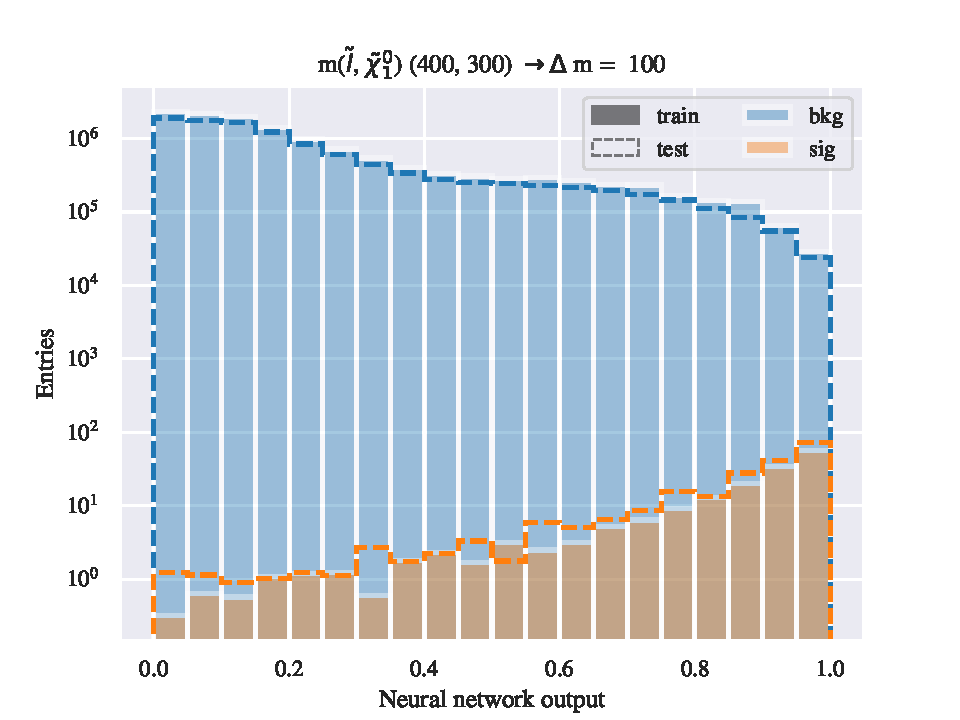
\includegraphics[width = \textwidth]{Figures/SlepSlep/ML/NN/Low_level/Low/scaled_train_test_395984.pdf}
        \caption{Direct slepton production.}
        \label{fig:SlepslepNNLow}
    \end{subfigure}
    \begin{subfigure}[t!]{0.49\textwidth}
        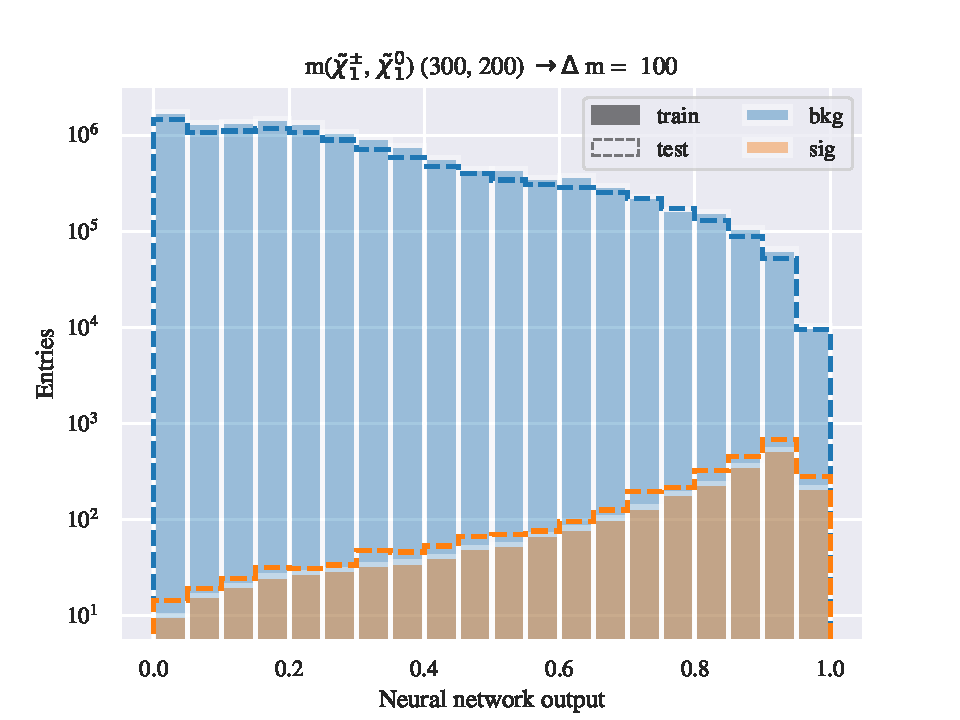
\includegraphics[width = \textwidth]{Figures/SlepSnu/NN/Low_level/Low/scaled_train_test_397115.pdf}
        \caption{Chargino production via $\Tilde{l}/\Tilde{\nu}$.}
        \label{fig:SlepsnuNNLow}
    \end{subfigure}    
    \begin{subfigure}[t!]{0.49\textwidth}
        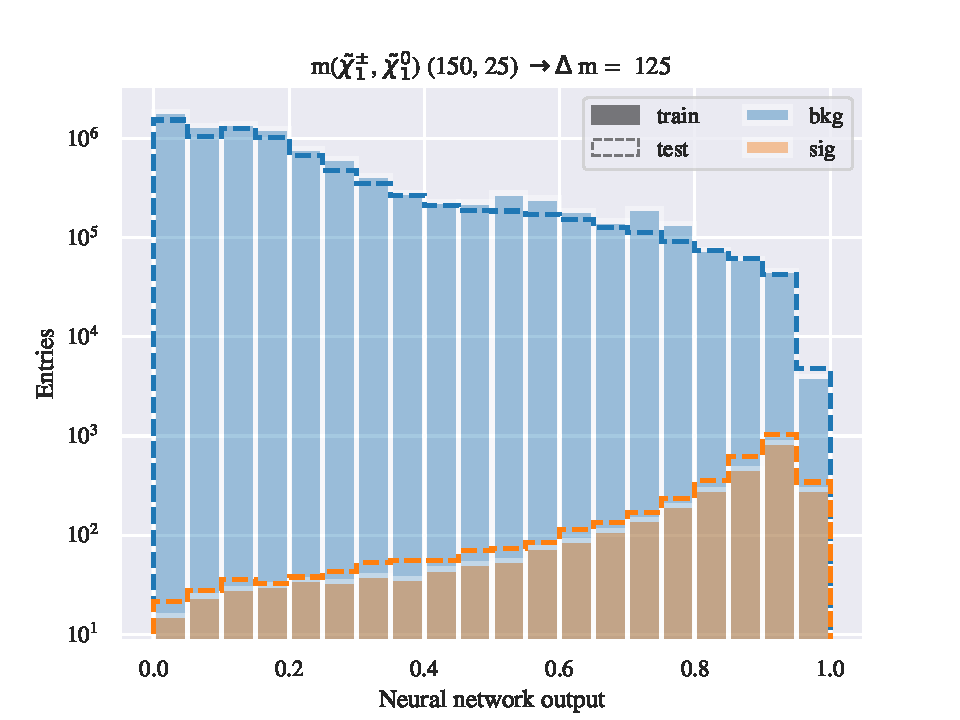
\includegraphics[width = \textwidth]{Figures/WW/NN/Low_level/Low/scaled_train_test_395268.pdf}
        \caption{Chargino production via $W^\pm$.}
        \label{fig:WWNNLow}
    \end{subfigure}
    \begin{subfigure}[t!]{0.49\textwidth}
        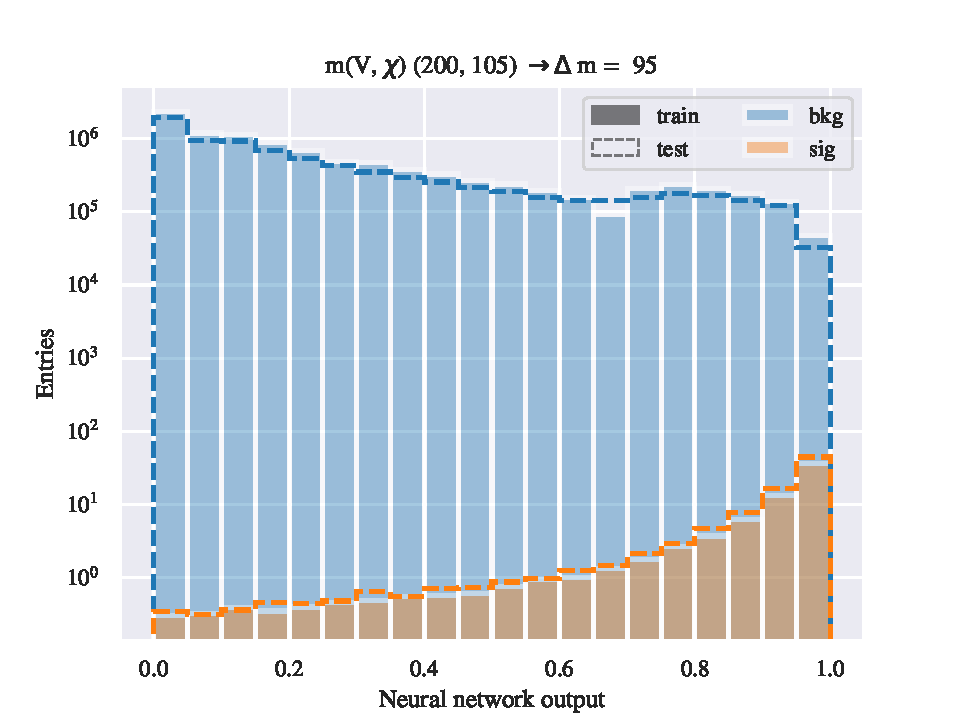
\includegraphics[width = \textwidth]{Figures/Mono_Z/ML/NN/Low_level/Low/scaled_train_test_310604.pdf}
        \caption{Mono-Z.}
        \label{fig:MonoZNNLow}
    \end{subfigure}
    \caption{Test vs train for low mass splittings done with the NN. Here the test set is scaled up to match the number of training events.}
    \label{fig:AllLowNN}
\end{figure}


\begin{figure}[H]
    \centering
    \begin{subfigure}[t!]{0.49\textwidth}
        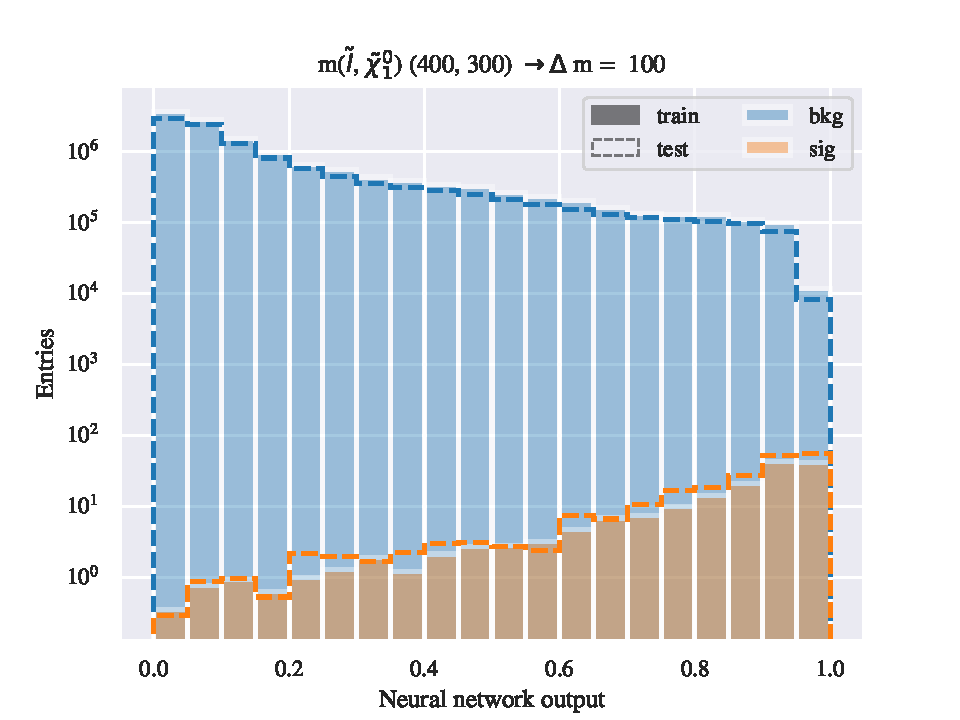
\includegraphics[width = \textwidth]{Figures/SlepSlep/ML/NN/High_level/Low/scaled_train_test_395984.pdf}
        \caption{Direct slepton production.}
        \label{fig:SlepslepNNLow}
    \end{subfigure}
    \begin{subfigure}[t!]{0.49\textwidth}
        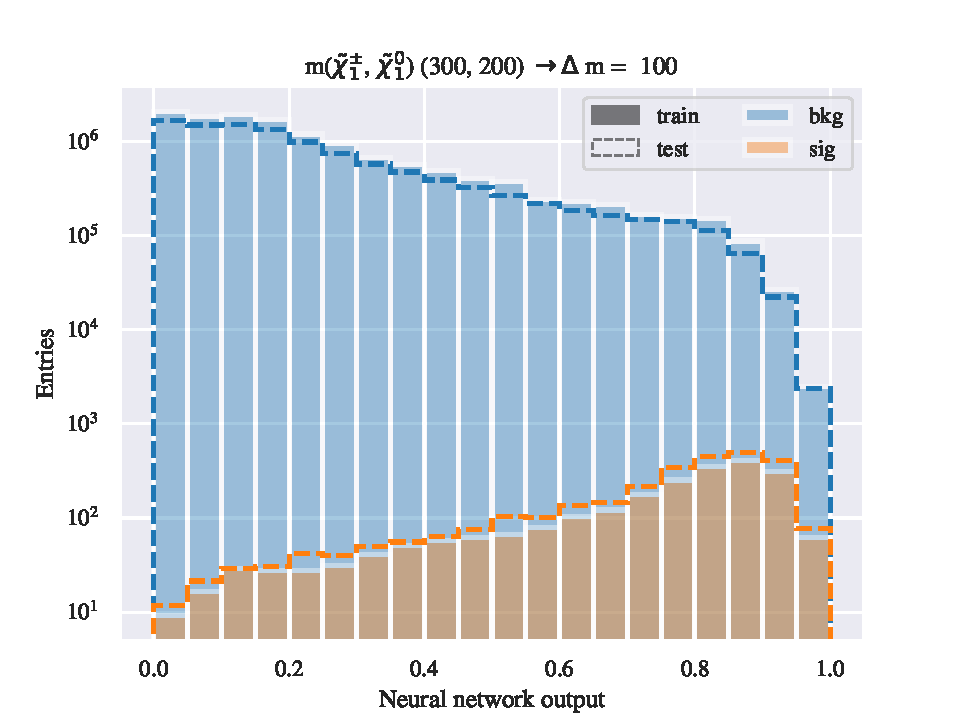
\includegraphics[width = \textwidth]{Figures/SlepSnu/NN/High_level/Low/scaled_train_test_397115.pdf}
        \caption{Chargino production via $\Tilde{l}/\Tilde{\nu}$.}
        \label{fig:SlepsnuNNLow}
    \end{subfigure}    
    \begin{subfigure}[t!]{0.49\textwidth}
        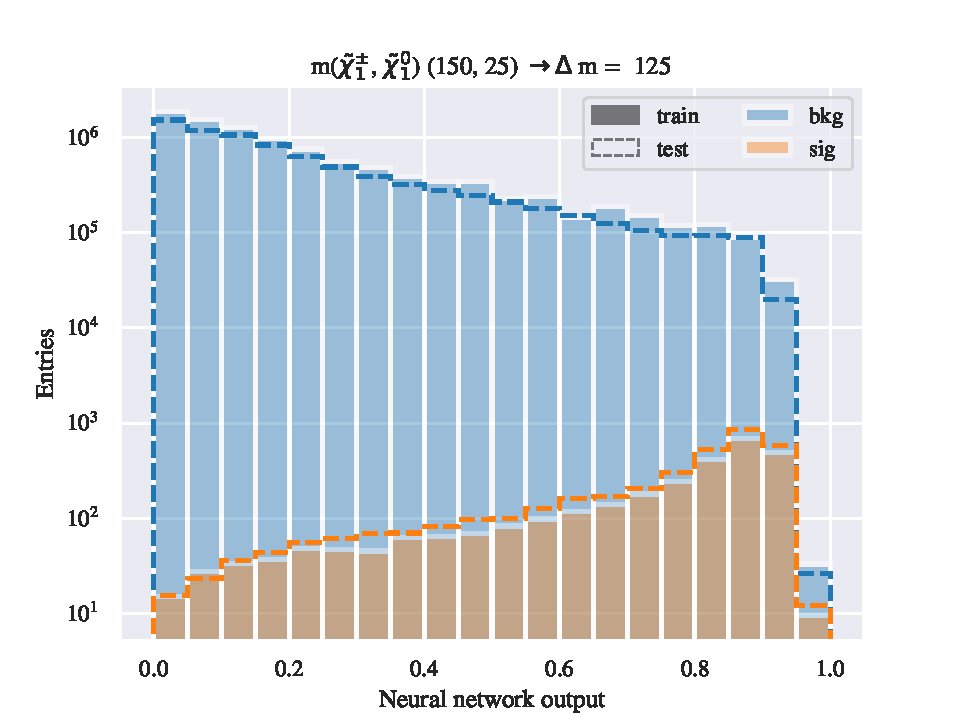
\includegraphics[width = \textwidth]{Figures/WW/NN/High_level/Low/scaled_train_test_395268.pdf}
        \caption{Chargino production via $W^\pm$.}
        \label{fig:WWNNLow}
    \end{subfigure}
    \begin{subfigure}[t!]{0.49\textwidth}
        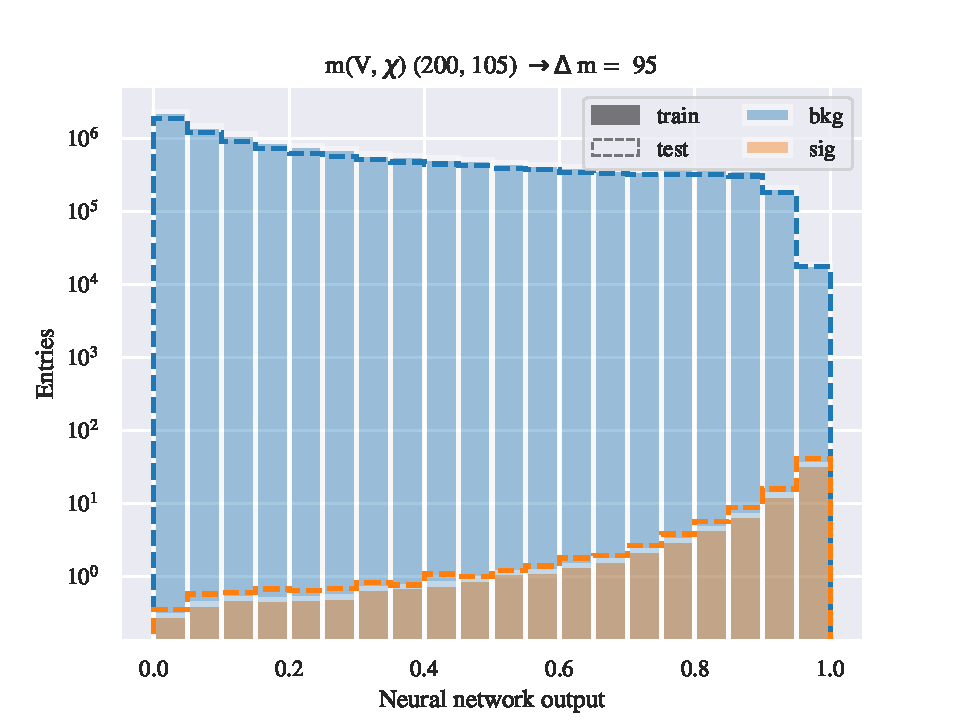
\includegraphics[width = \textwidth]{Figures/Mono_Z/ML/NN/High_level/Low/scaled_train_test_310604.pdf}
        \caption{Mono-Z.}
        \label{fig:MonoZNNLow}
    \end{subfigure}
    \caption{Test vs train for low mass splittings done with the NN. Here the test set is scaled up to match the number of training events.}
    \label{fig:AllLowNN}
\end{figure}


\begin{figure}[H]
    \centering
    \begin{subfigure}[t!]{0.49\textwidth}
        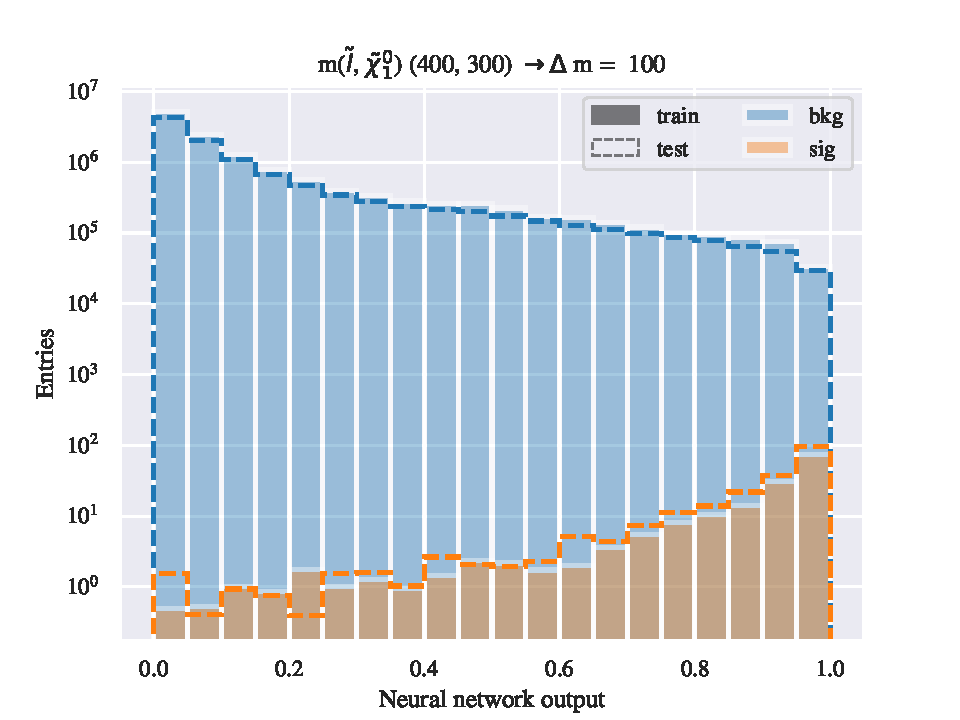
\includegraphics[width = \textwidth]{Figures/SlepSlep/ML/NN/All_level/Low/scaled_train_test_395984.pdf}
        \caption{Direct slepton production.}
        \label{fig:SlepslepNNLow}
    \end{subfigure}
    \begin{subfigure}[t!]{0.49\textwidth}
        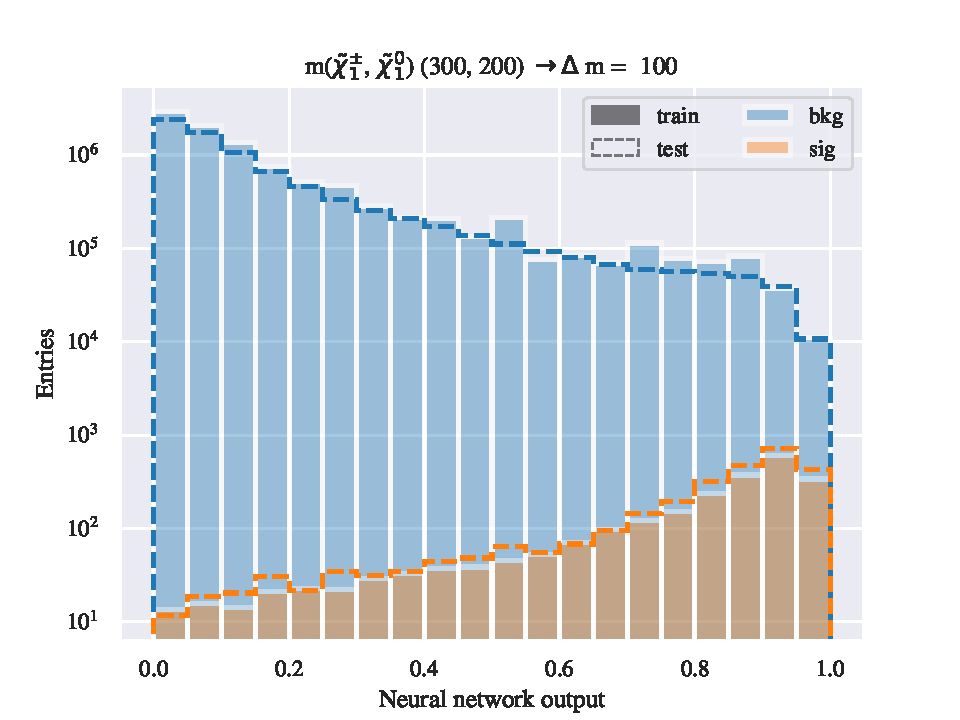
\includegraphics[width = \textwidth]{Figures/SlepSnu/NN/All_level/Low/scaled_train_test_397115.pdf}
        \caption{Chargino production via $\Tilde{l}/\Tilde{\nu}$.}
        \label{fig:SlepsnuNNLow}
    \end{subfigure}    
    \begin{subfigure}[t!]{0.49\textwidth}
        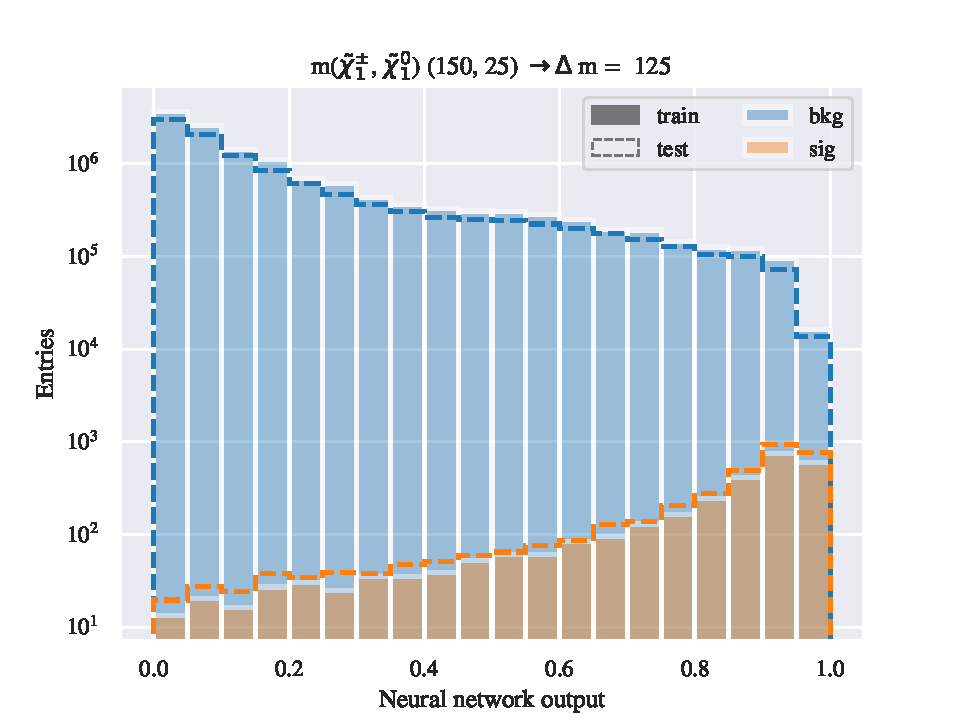
\includegraphics[width = \textwidth]{Figures/WW/NN/All_level/Low/scaled_train_test_395268.pdf}
        \caption{Chargino production via $W^\pm$.}
        \label{fig:WWNNLow}
    \end{subfigure}
    \begin{subfigure}[t!]{0.49\textwidth}
        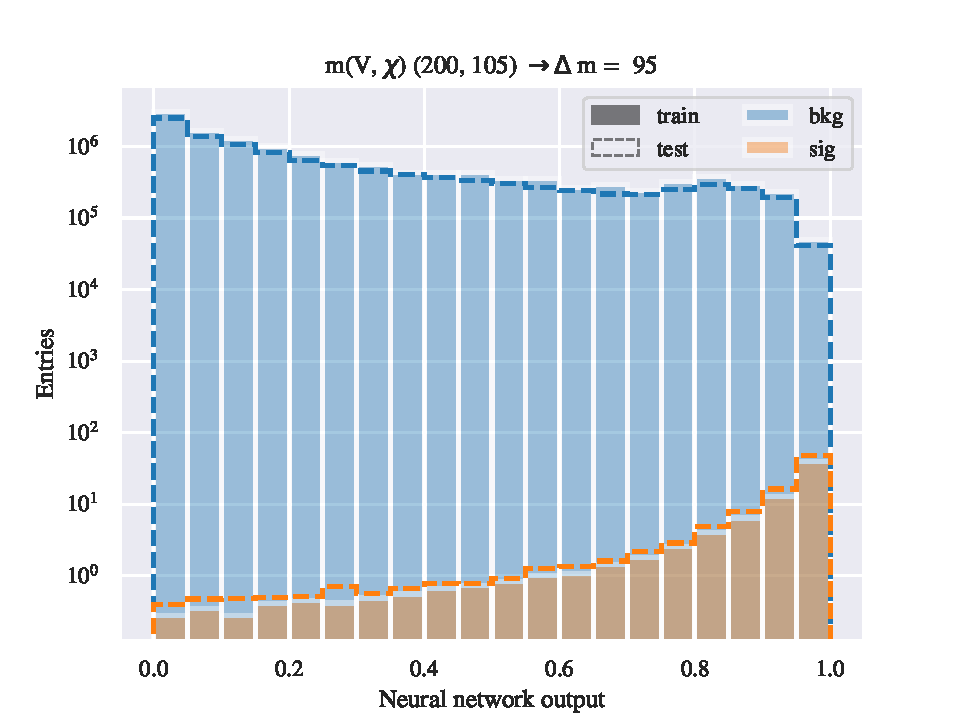
\includegraphics[width = \textwidth]{Figures/Mono_Z/ML/NN/All_level/Low/scaled_train_test_310604.pdf}
        \caption{Mono-Z.}
        \label{fig:MonoZNNLow}
    \end{subfigure}
    \caption{Test vs train for low mass splittings done with the NN. Here the test set is scaled up to match the number of training events.}
    \label{fig:AllLowNN}
\end{figure}














\subsubsection{Intermediate mass splittings}



\begin{figure}[H]
    \centering
    \begin{subfigure}[t!]{0.49\textwidth}
        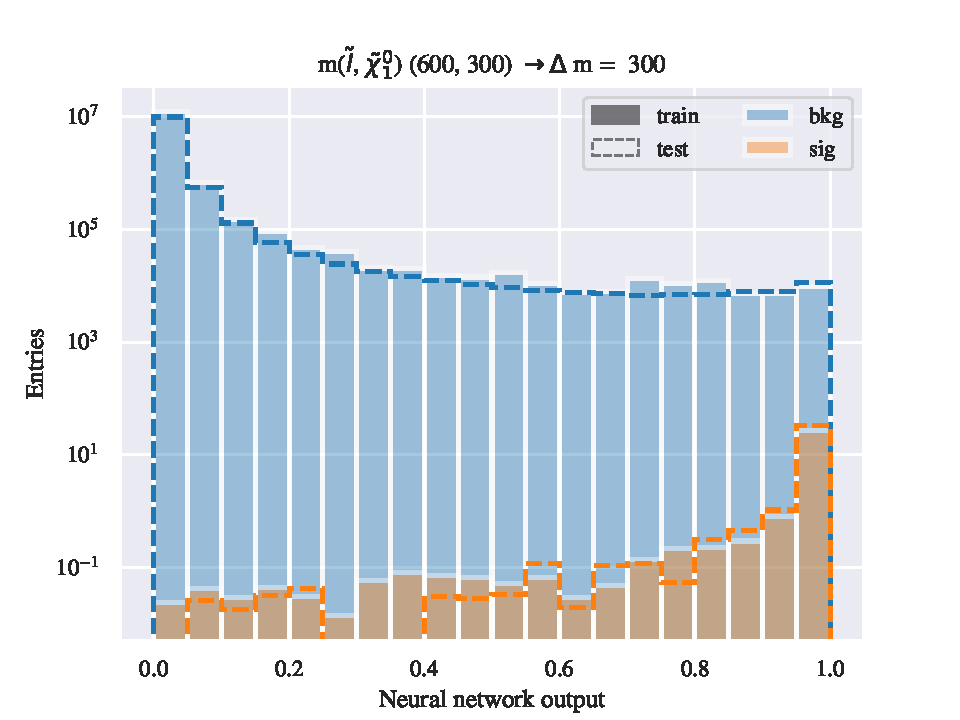
\includegraphics[width = \textwidth]{Figures/SlepSlep/ML/NN/Low_level/Inter/scaled_train_test_396014.pdf}
        \caption{Direct slepton production.}
        \label{fig:SlepslepNNLow}
    \end{subfigure}
    \begin{subfigure}[t!]{0.49\textwidth}
        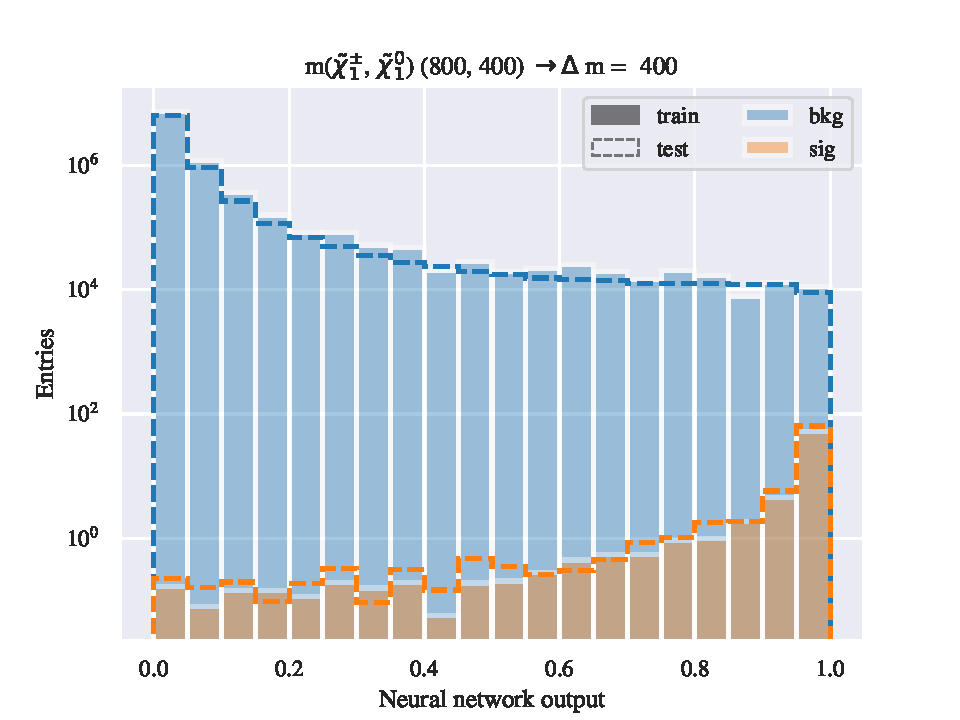
\includegraphics[width = \textwidth]{Figures/SlepSnu/NN/Low_level/Inter/scaled_train_test_397150.pdf}
        \caption{Chargino production via $\Tilde{l}/\Tilde{\nu}$.}
        \label{fig:SlepsnuNNLow}
    \end{subfigure}    
    \begin{subfigure}[t!]{0.49\textwidth}
        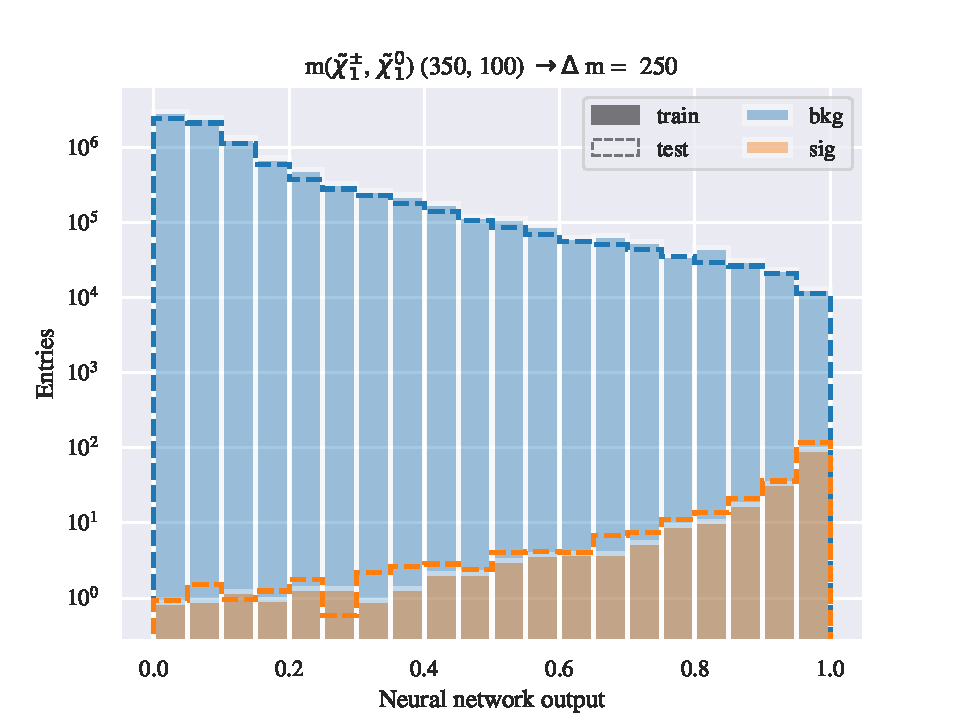
\includegraphics[width = \textwidth]{Figures/WW/NN/Low_level/Inter/scaled_train_test_395320.pdf}
        \caption{Chargino production via $W^\pm$.}
        \label{fig:WWNNLow}
    \end{subfigure}
    \begin{subfigure}[t!]{0.49\textwidth}
        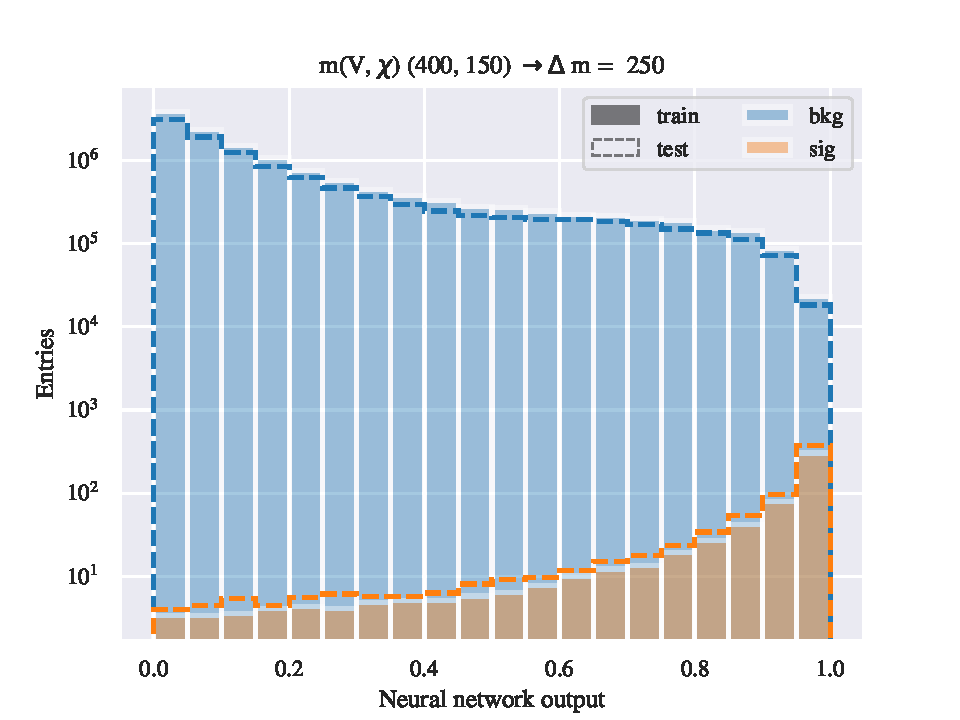
\includegraphics[width = \textwidth]{Figures/Mono_Z/ML/NN/Low_level/Inter/scaled_train_test_310613.pdf}
        \caption{Mono-Z.}
        \label{fig:MonoZNNLow}
    \end{subfigure}
    \caption{Test vs train for low mass splittings done with the NN. Here the test set is scaled up to match the number of training events.}
    \label{fig:AllLowNN}
\end{figure}


\begin{figure}[H]
    \centering
    \begin{subfigure}[t!]{0.49\textwidth}
        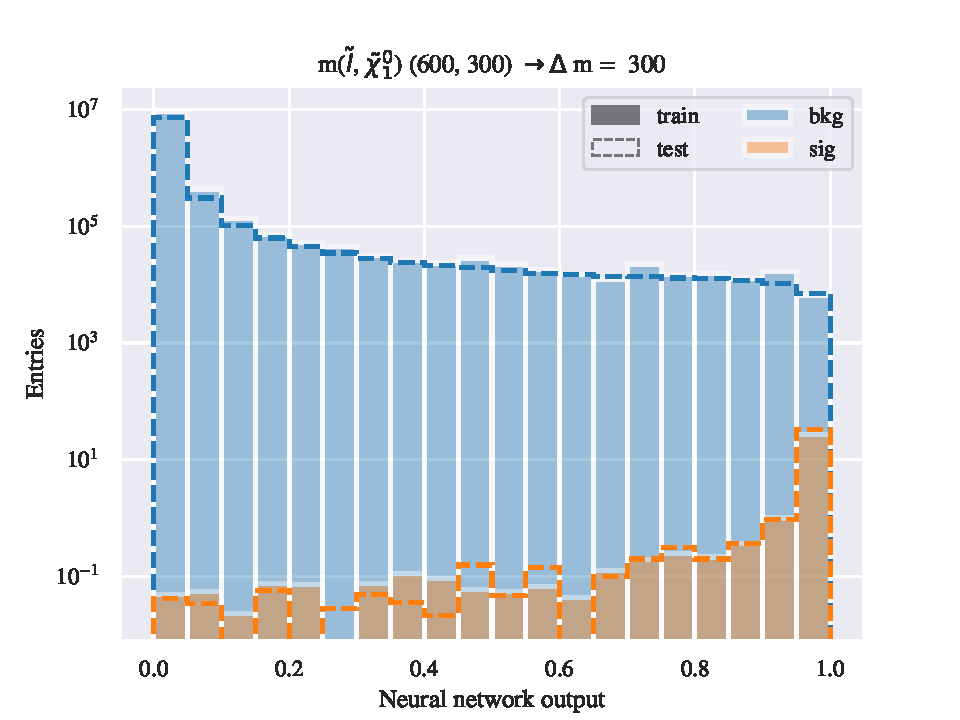
\includegraphics[width = \textwidth]{Figures/SlepSlep/ML/NN/High_level/Inter/scaled_train_test_396014.pdf}
        \caption{Direct slepton production.}
        \label{fig:SlepslepNNLow}
    \end{subfigure}
    \begin{subfigure}[t!]{0.49\textwidth}
        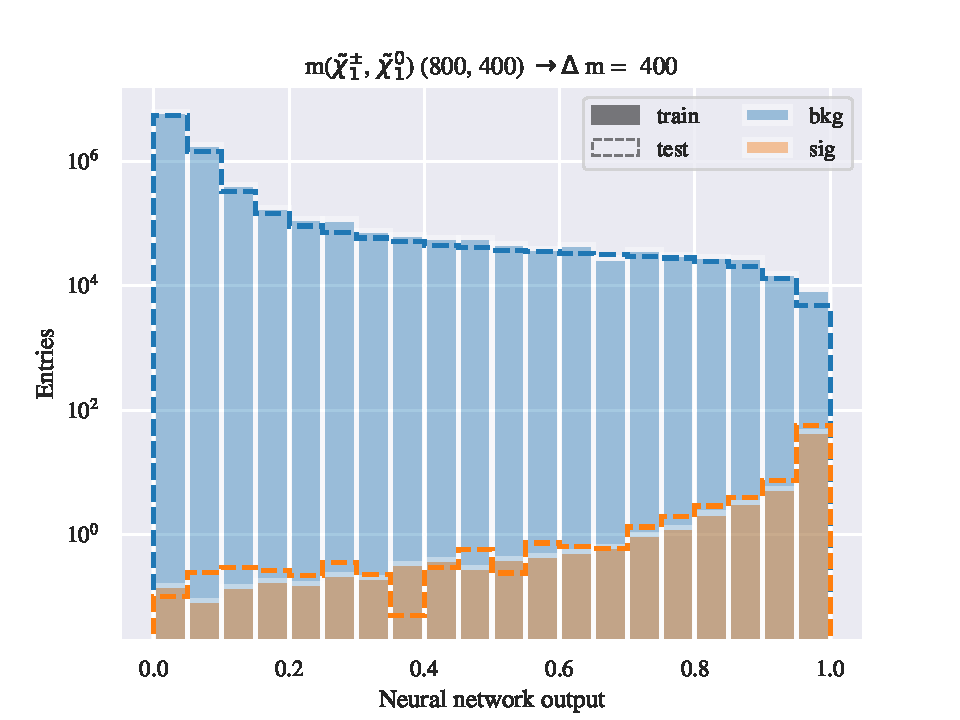
\includegraphics[width = \textwidth]{Figures/SlepSnu/NN/High_level/Inter/scaled_train_test_397150.pdf}
        \caption{Chargino production via $\Tilde{l}/\Tilde{\nu}$.}
        \label{fig:SlepsnuNNLow}
    \end{subfigure}    
    \begin{subfigure}[t!]{0.49\textwidth}
        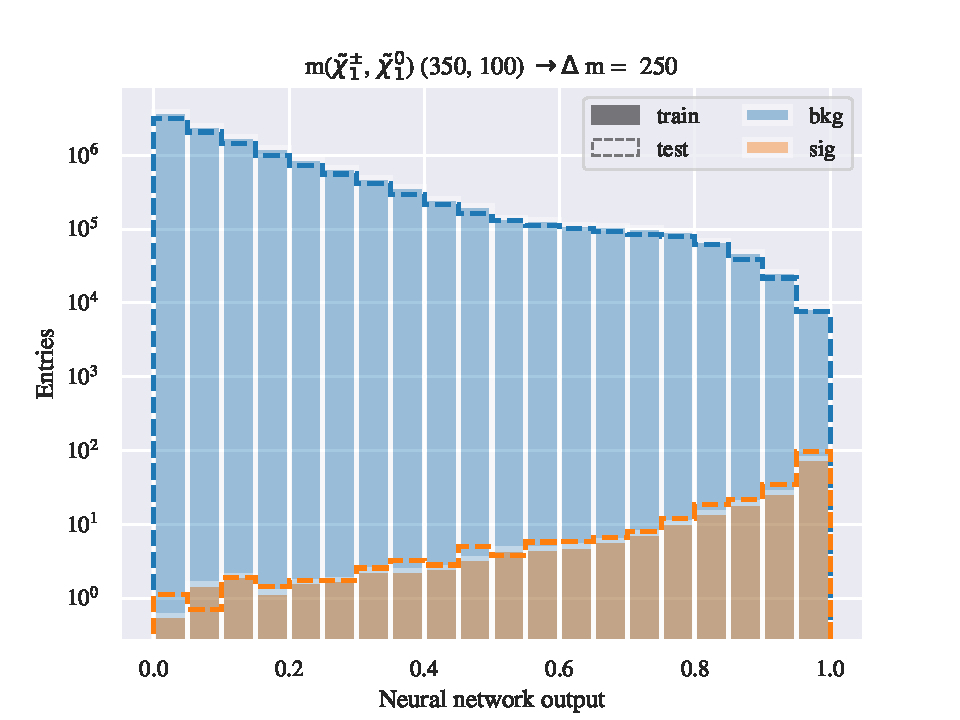
\includegraphics[width = \textwidth]{Figures/WW/NN/High_level/Inter/scaled_train_test_395320.pdf}
        \caption{Chargino production via $W^\pm$.}
        \label{fig:WWNNLow}
    \end{subfigure}
    \begin{subfigure}[t!]{0.49\textwidth}
        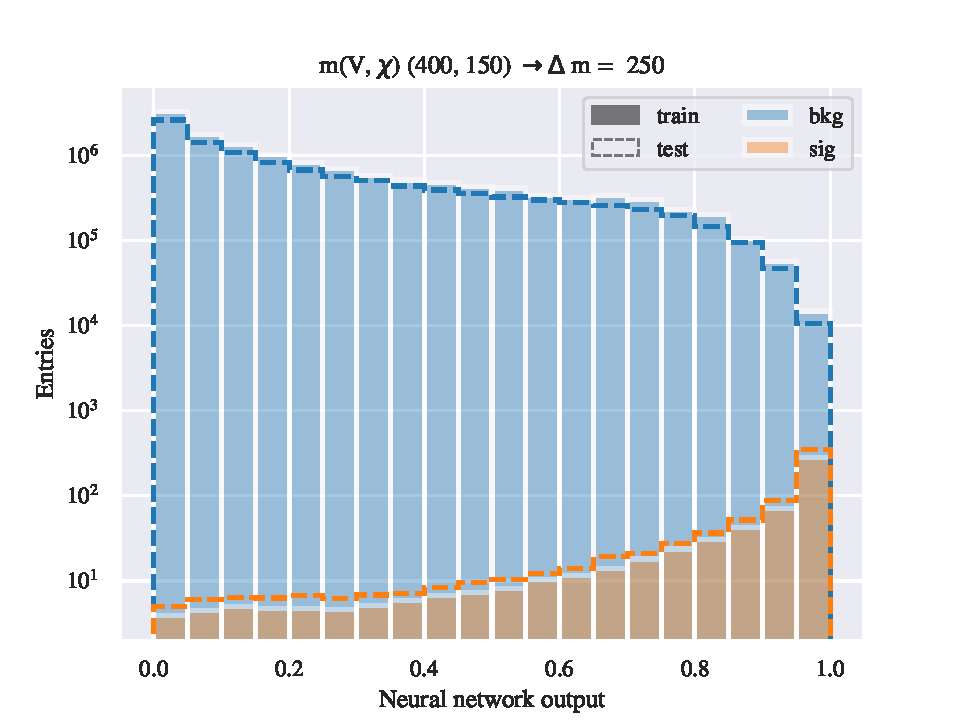
\includegraphics[width = \textwidth]{Figures/Mono_Z/ML/NN/High_level/Inter/scaled_train_test_310613.pdf}
        \caption{Mono-Z.}
        \label{fig:MonoZNNLow}
    \end{subfigure}
    \caption{Test vs train for low mass splittings done with the NN. Here the test set is scaled up to match the number of training events.}
    \label{fig:AllLowNN}
\end{figure}


\begin{figure}[H]
    \centering
    \begin{subfigure}[t!]{0.49\textwidth}
        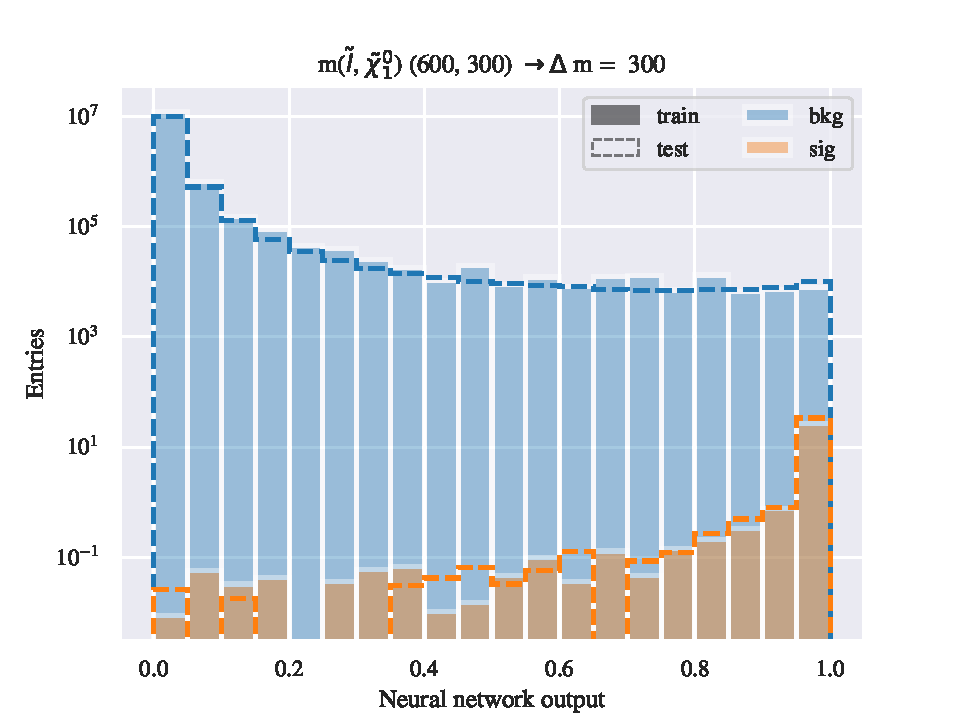
\includegraphics[width = \textwidth]{Figures/SlepSlep/ML/NN/All_level/Inter/scaled_train_test_396014.pdf}
        \caption{Direct slepton production.}
        \label{fig:SlepslepNNLow}
    \end{subfigure}
    \begin{subfigure}[t!]{0.49\textwidth}
        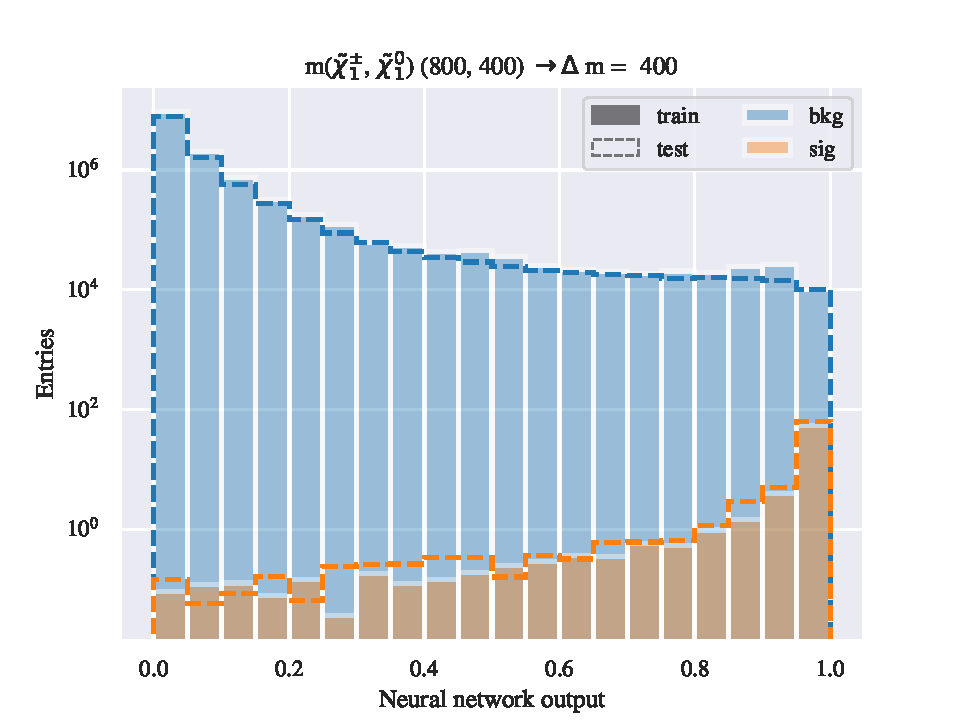
\includegraphics[width = \textwidth]{Figures/SlepSnu/NN/All_level/Inter/scaled_train_test_397150.pdf}
        \caption{Chargino production via $\Tilde{l}/\Tilde{\nu}$.}
        \label{fig:SlepsnuNNLow}
    \end{subfigure}    
    \begin{subfigure}[t!]{0.49\textwidth}
        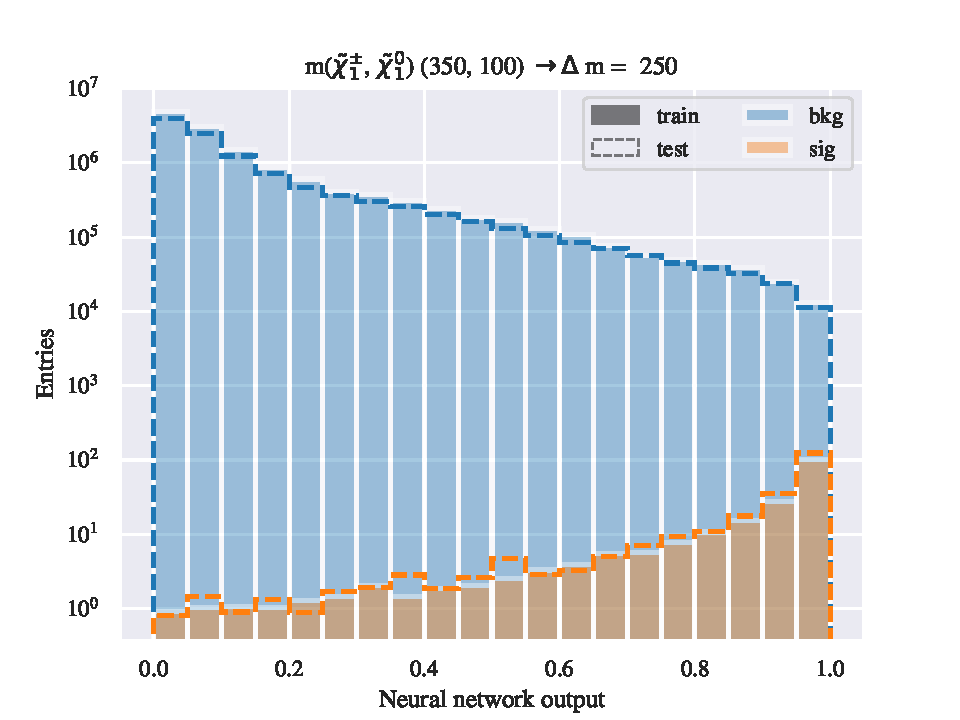
\includegraphics[width = \textwidth]{Figures/WW/NN/All_level/Inter/scaled_train_test_395320.pdf}
        \caption{Chargino production via $W^\pm$.}
        \label{fig:WWNNLow}
    \end{subfigure}
    \begin{subfigure}[t!]{0.49\textwidth}
        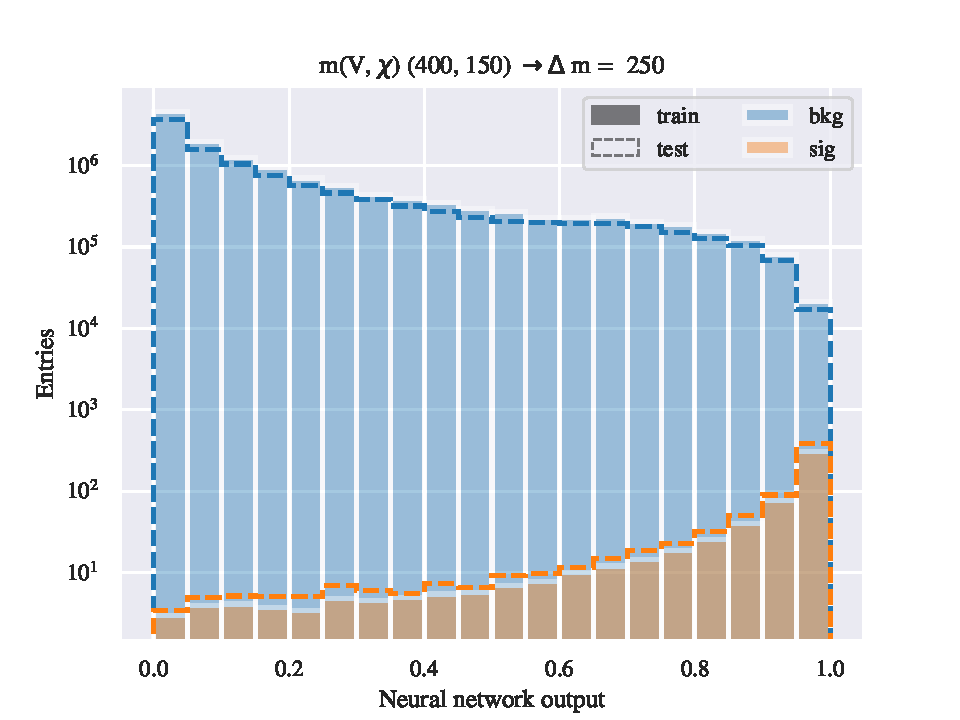
\includegraphics[width = \textwidth]{Figures/Mono_Z/ML/NN/All_level/Inter/scaled_train_test_310613.pdf}
        \caption{Mono-Z.}
        \label{fig:MonoZNNLow}
    \end{subfigure}
    \caption{Test vs train for low mass splittings done with the NN. Here the test set is scaled up to match the number of training events.}
    \label{fig:AllLowNN}
\end{figure}



















\subsubsection{High mass splittings}

\begin{figure}[H]
    \centering
    \begin{subfigure}[t!]{0.49\textwidth}
        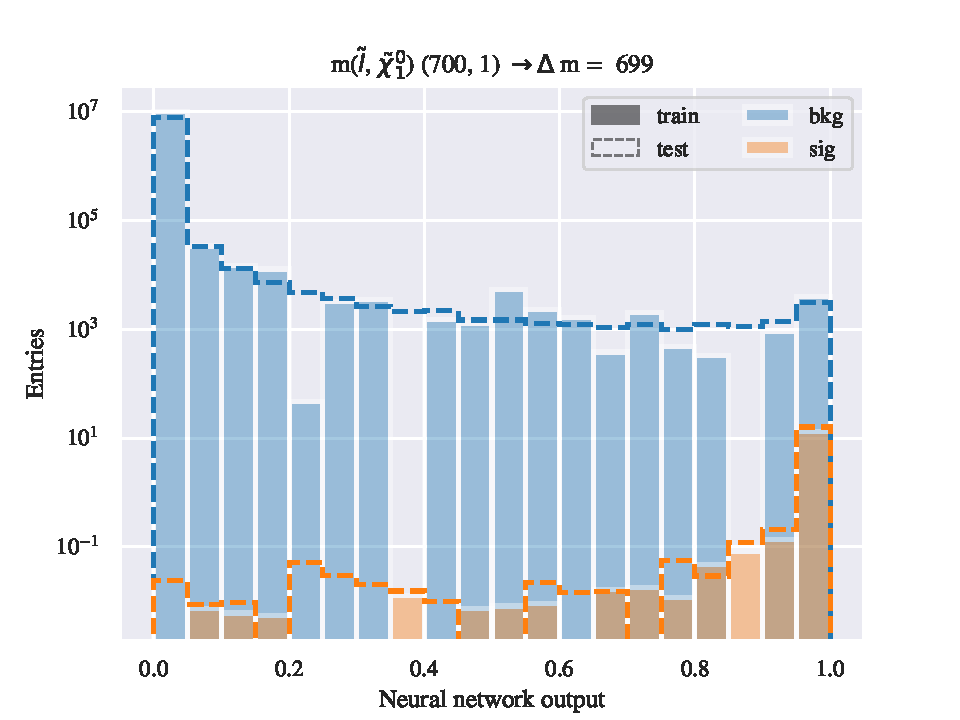
\includegraphics[width = \textwidth]{Figures/SlepSlep/ML/NN/Low_level/High/scaled_train_test_396033.pdf}
        \caption{Direct slepton production.}
        \label{fig:SlepslepNNLow}
    \end{subfigure}
    \begin{subfigure}[t!]{0.49\textwidth}
        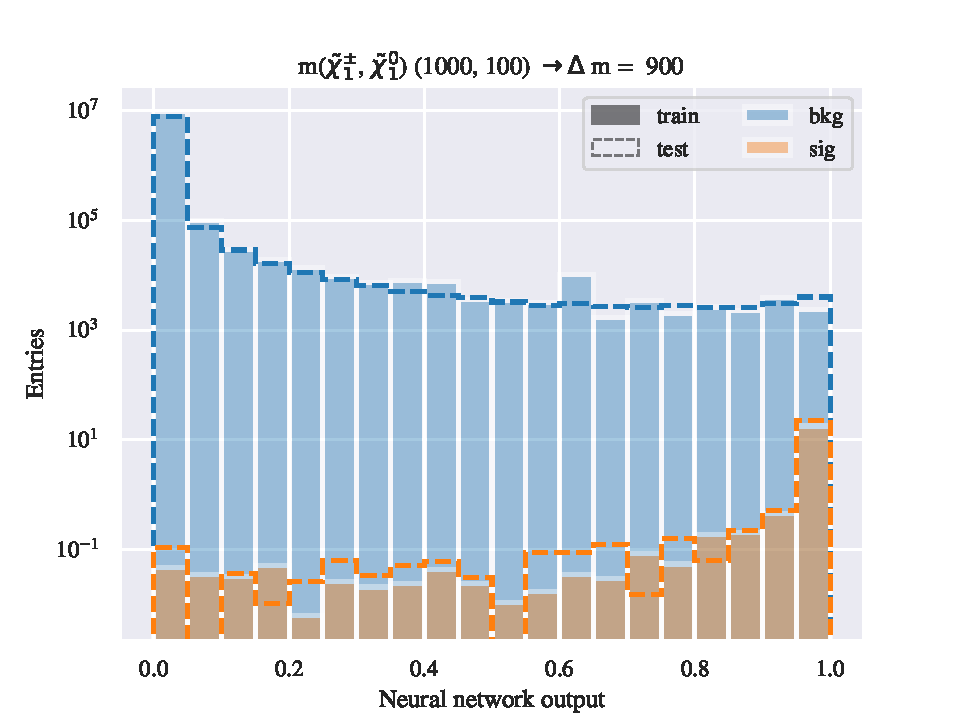
\includegraphics[width = \textwidth]{Figures/SlepSnu/NN/Low_level/High/scaled_train_test_397169.pdf}
        \caption{Chargino production via $\Tilde{l}/\Tilde{\nu}$.}
        \label{fig:SlepsnuNNLow}
    \end{subfigure}    
    \begin{subfigure}[t!]{0.49\textwidth}
        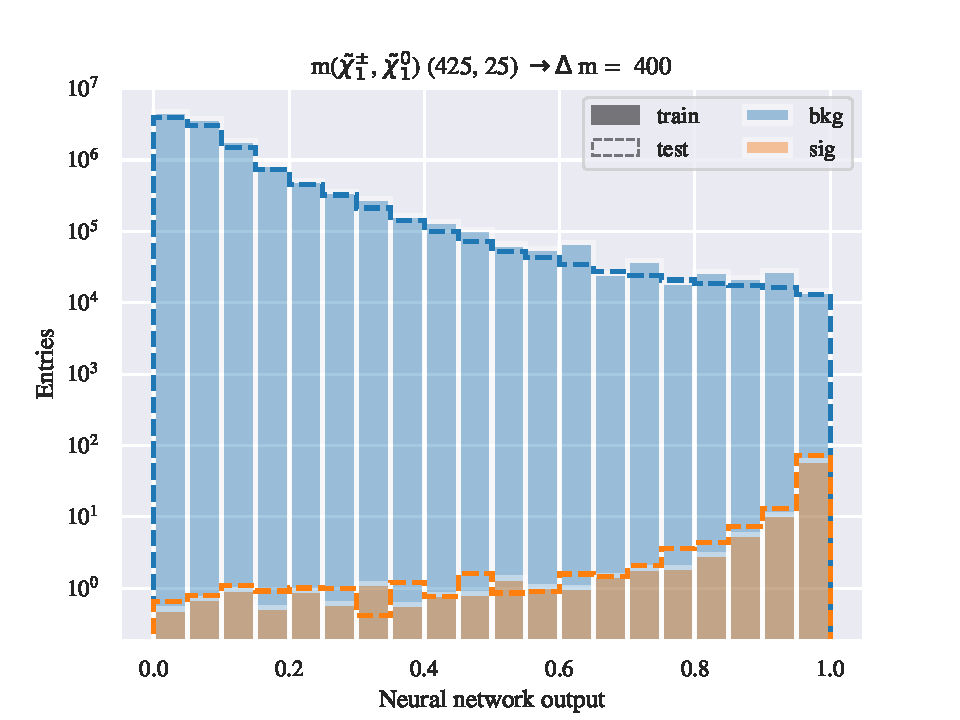
\includegraphics[width = \textwidth]{Figures/WW/NN/Low_level/High/scaled_train_test_395330.pdf}
        \caption{Chargino production via $W^\pm$.}
        \label{fig:WWNNLow}
    \end{subfigure}
    \begin{subfigure}[t!]{0.49\textwidth}
        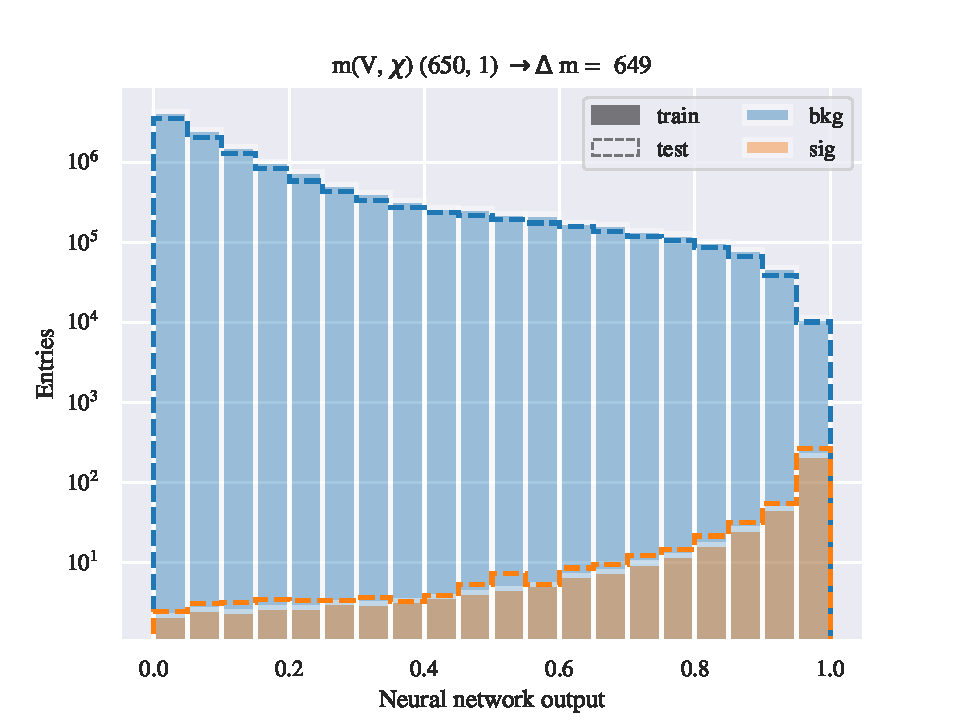
\includegraphics[width = \textwidth]{Figures/Mono_Z/ML/NN/Low_level/High/scaled_train_test_310617.pdf}
        \caption{Mono-Z.}
        \label{fig:MonoZNNLow}
    \end{subfigure}
    \caption{Test vs train for low mass splittings done with the NN. Here the test set is scaled up to match the number of training events.}
    \label{fig:AllLowNN}
\end{figure}


\begin{figure}[H]
    \centering
    \begin{subfigure}[t!]{0.49\textwidth}
        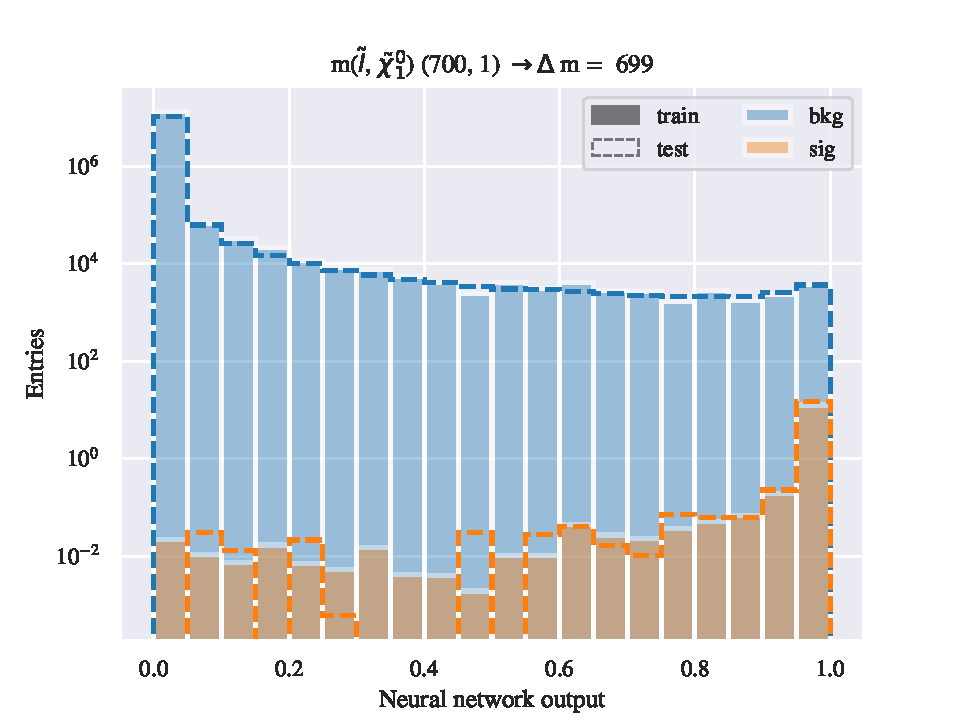
\includegraphics[width = \textwidth]{Figures/SlepSlep/ML/NN/High_level/High/scaled_train_test_396033.pdf}
        \caption{Direct slepton production.}
        \label{fig:SlepslepNNLow}
    \end{subfigure}
    \begin{subfigure}[t!]{0.49\textwidth}
        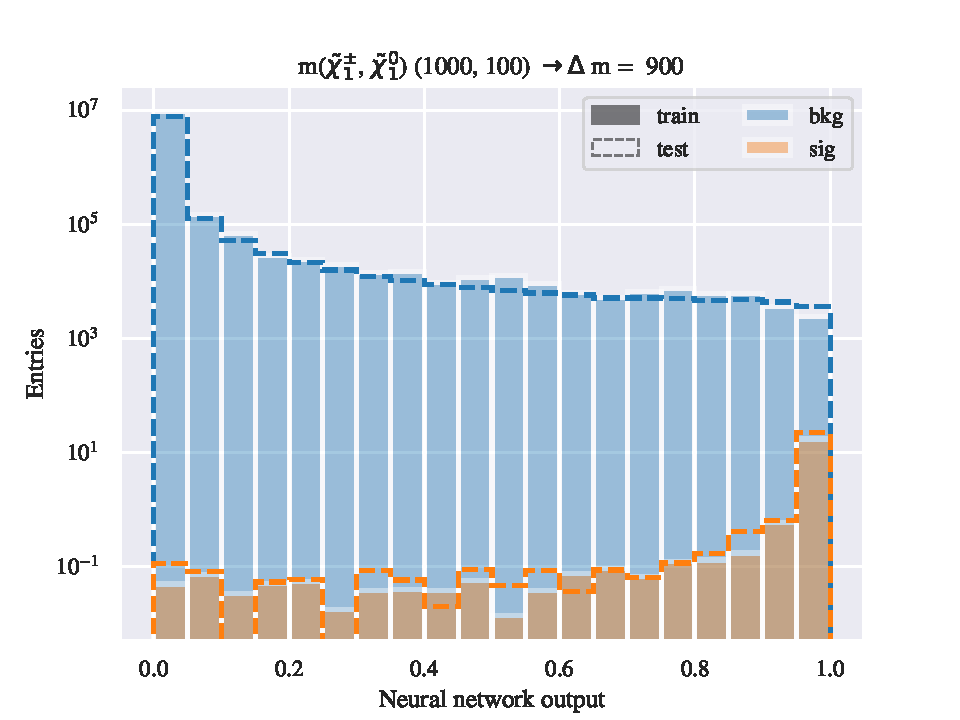
\includegraphics[width = \textwidth]{Figures/SlepSnu/NN/High_level/High/scaled_train_test_397169.pdf}
        \caption{Chargino production via $\Tilde{l}/\Tilde{\nu}$.}
        \label{fig:SlepsnuNNLow}
    \end{subfigure}    
    \begin{subfigure}[t!]{0.49\textwidth}
        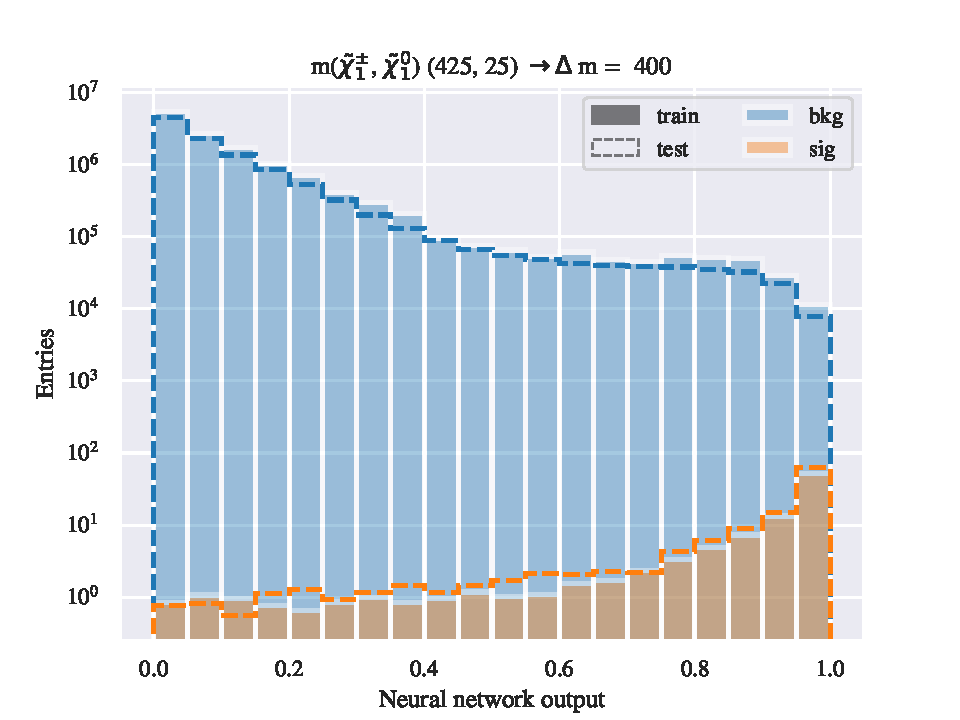
\includegraphics[width = \textwidth]{Figures/WW/NN/High_level/High/scaled_train_test_395330.pdf}
        \caption{Chargino production via $W^\pm$.}
        \label{fig:WWNNLow}
    \end{subfigure}
    \begin{subfigure}[t!]{0.49\textwidth}
        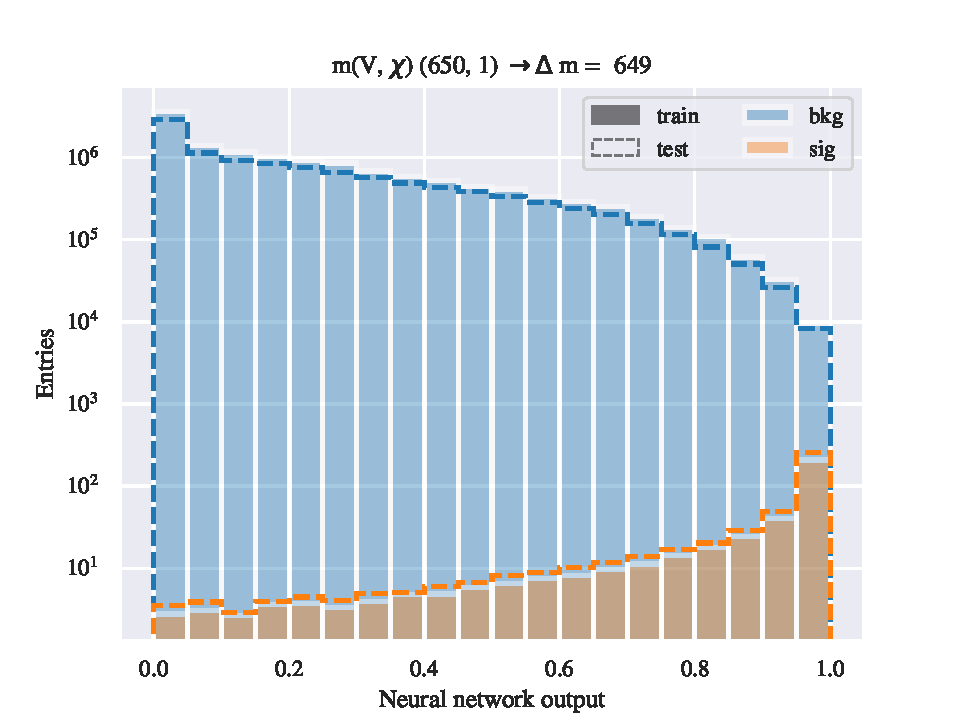
\includegraphics[width = \textwidth]{Figures/Mono_Z/ML/NN/High_level/High/scaled_train_test_310617.pdf}
        \caption{Mono-Z.}
        \label{fig:MonoZNNLow}
    \end{subfigure}
    \caption{Test vs train for low mass splittings done with the NN. Here the test set is scaled up to match the number of training events.}
    \label{fig:AllLowNN}
\end{figure}


\begin{figure}[H]
    \centering
    \begin{subfigure}[t!]{0.49\textwidth}
        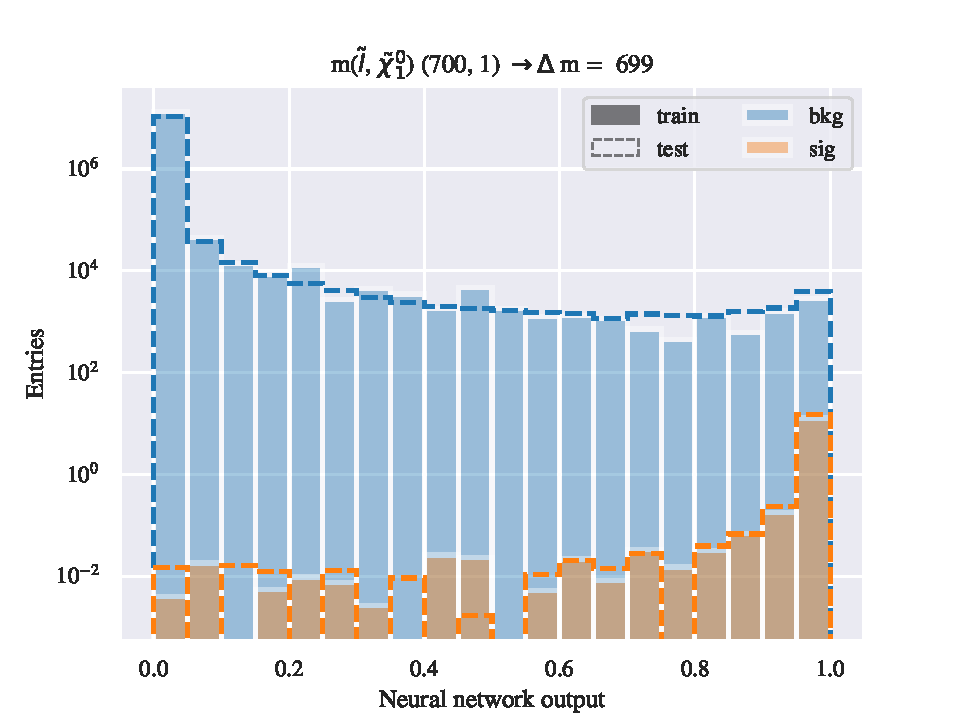
\includegraphics[width = \textwidth]{Figures/SlepSlep/ML/NN/All_level/High/scaled_train_test_396033.pdf}
        \caption{Direct slepton production.}
        \label{fig:SlepslepNNLow}
    \end{subfigure}
    \begin{subfigure}[t!]{0.49\textwidth}
        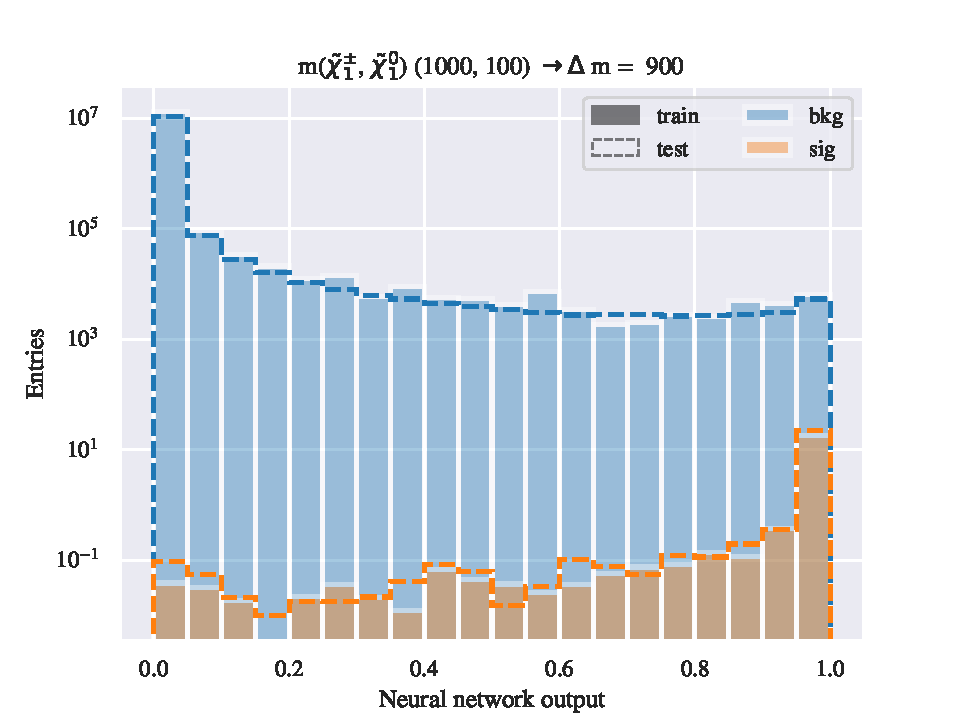
\includegraphics[width = \textwidth]{Figures/SlepSnu/NN/All_level/High/scaled_train_test_397169.pdf}
        \caption{Chargino production via $\Tilde{l}/\Tilde{\nu}$.}
        \label{fig:SlepsnuNNLow}
    \end{subfigure}    
    \begin{subfigure}[t!]{0.49\textwidth}
        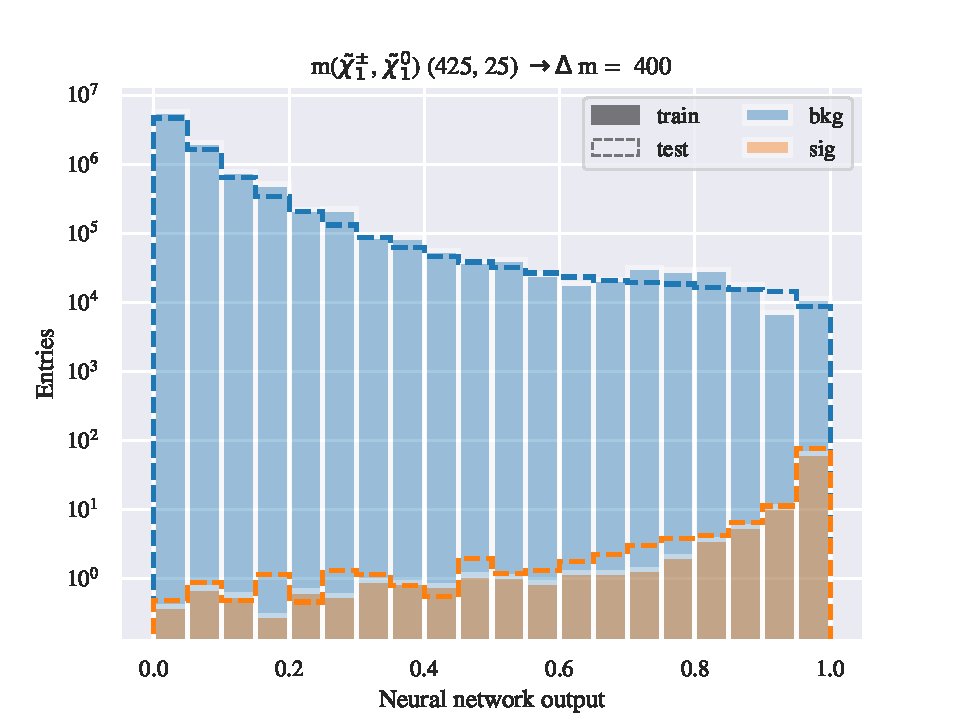
\includegraphics[width = \textwidth]{Figures/WW/NN/All_level/High/scaled_train_test_395330.pdf}
        \caption{Chargino production via $W^\pm$.}
        \label{fig:WWNNLow}
    \end{subfigure}
    \begin{subfigure}[t!]{0.49\textwidth}
        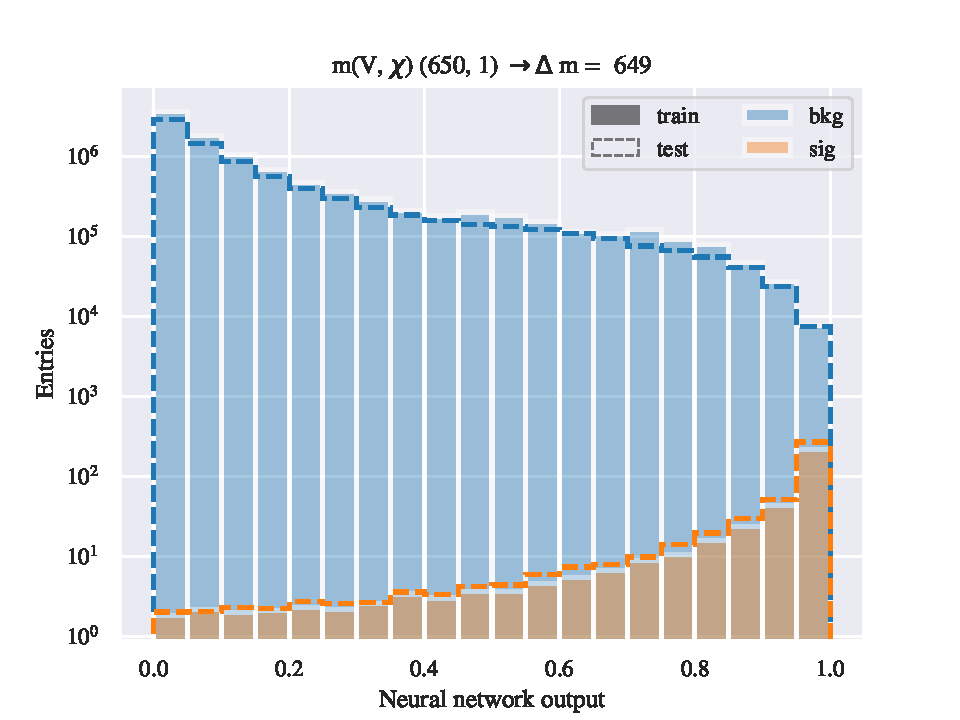
\includegraphics[width = \textwidth]{Figures/Mono_Z/ML/NN/All_level/High/scaled_train_test_310617.pdf}
        \caption{Mono-Z.}
        \label{fig:MonoZNNLow}
    \end{subfigure}
    \caption{Test vs train for low mass splittings done with the NN. Here the test set is scaled up to match the number of training events.}
    \label{fig:AllLowNN}
\end{figure}






















\begin{figure}[H]
    \centering
    \begin{subfigure}[t!]{0.49\textwidth}
        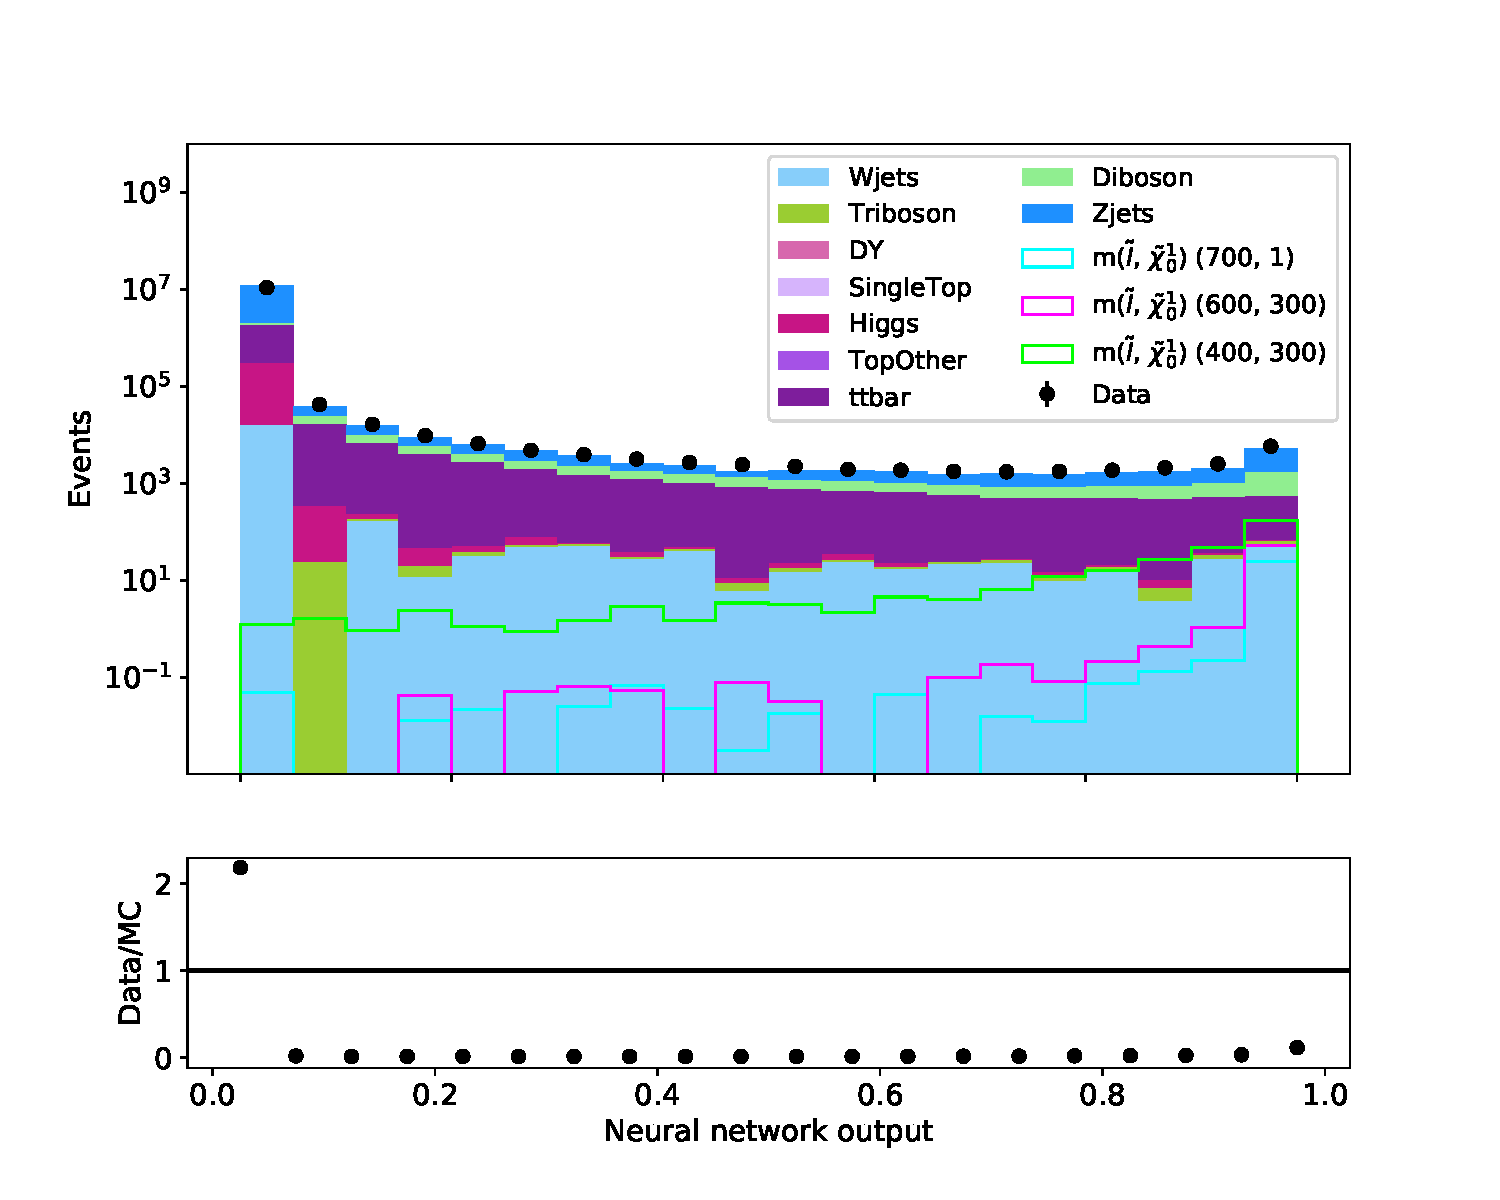
\includegraphics[width = \textwidth]{Figures/Stacked/stackedplot_NN_All_level_slepslep.pdf}
        \caption{Direct slepton production.}
        \label{fig:SlepslepNNLow}
    \end{subfigure}
    \begin{subfigure}[t!]{0.49\textwidth}
        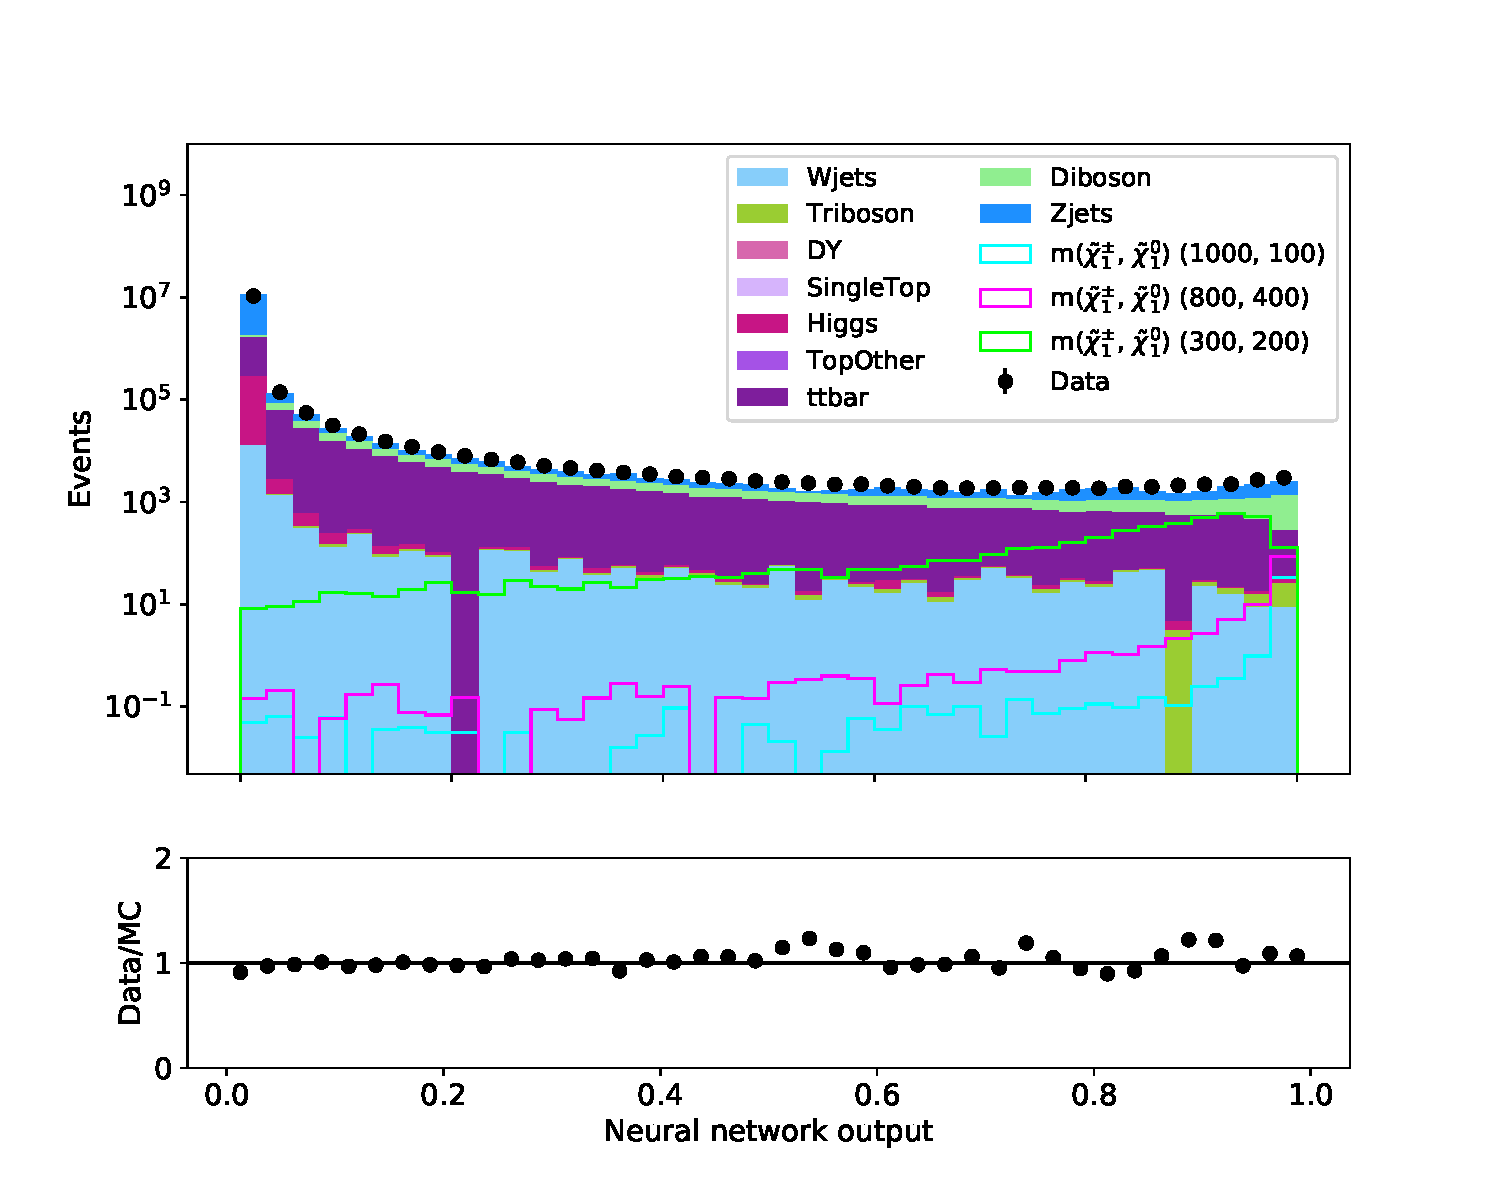
\includegraphics[width = \textwidth]{Figures/Stacked/stackedplot_NN_All_level_slepsnu.pdf}
        \caption{Chargino production via $\Tilde{l}/\Tilde{\nu}$.}
        \label{fig:SlepsnuNNLow}
    \end{subfigure}      
    \begin{subfigure}[t!]{0.49\textwidth}
        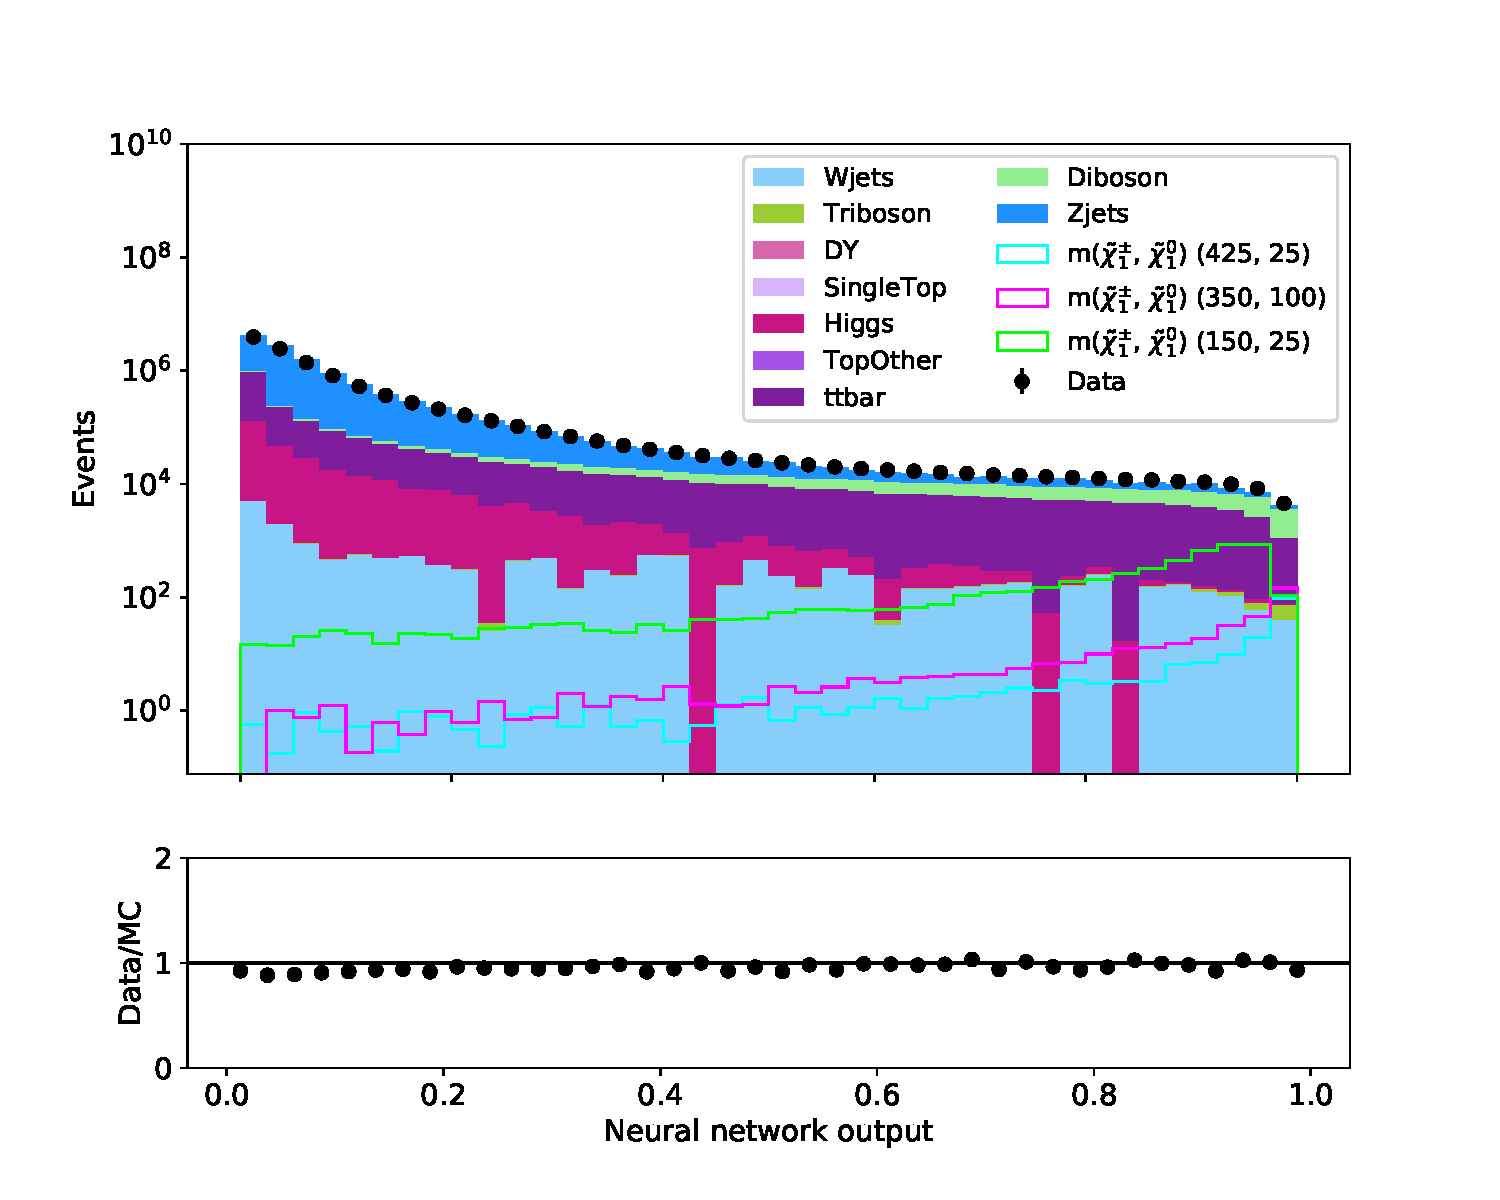
\includegraphics[width = \textwidth]{Figures/Stacked/stackedplot_NN_All_level_WW.pdf}
        \caption{Chargino production via $W^\pm$.}
        \label{fig:WWNNLow}
    \end{subfigure}
    \begin{subfigure}[t!]{0.49\textwidth}
        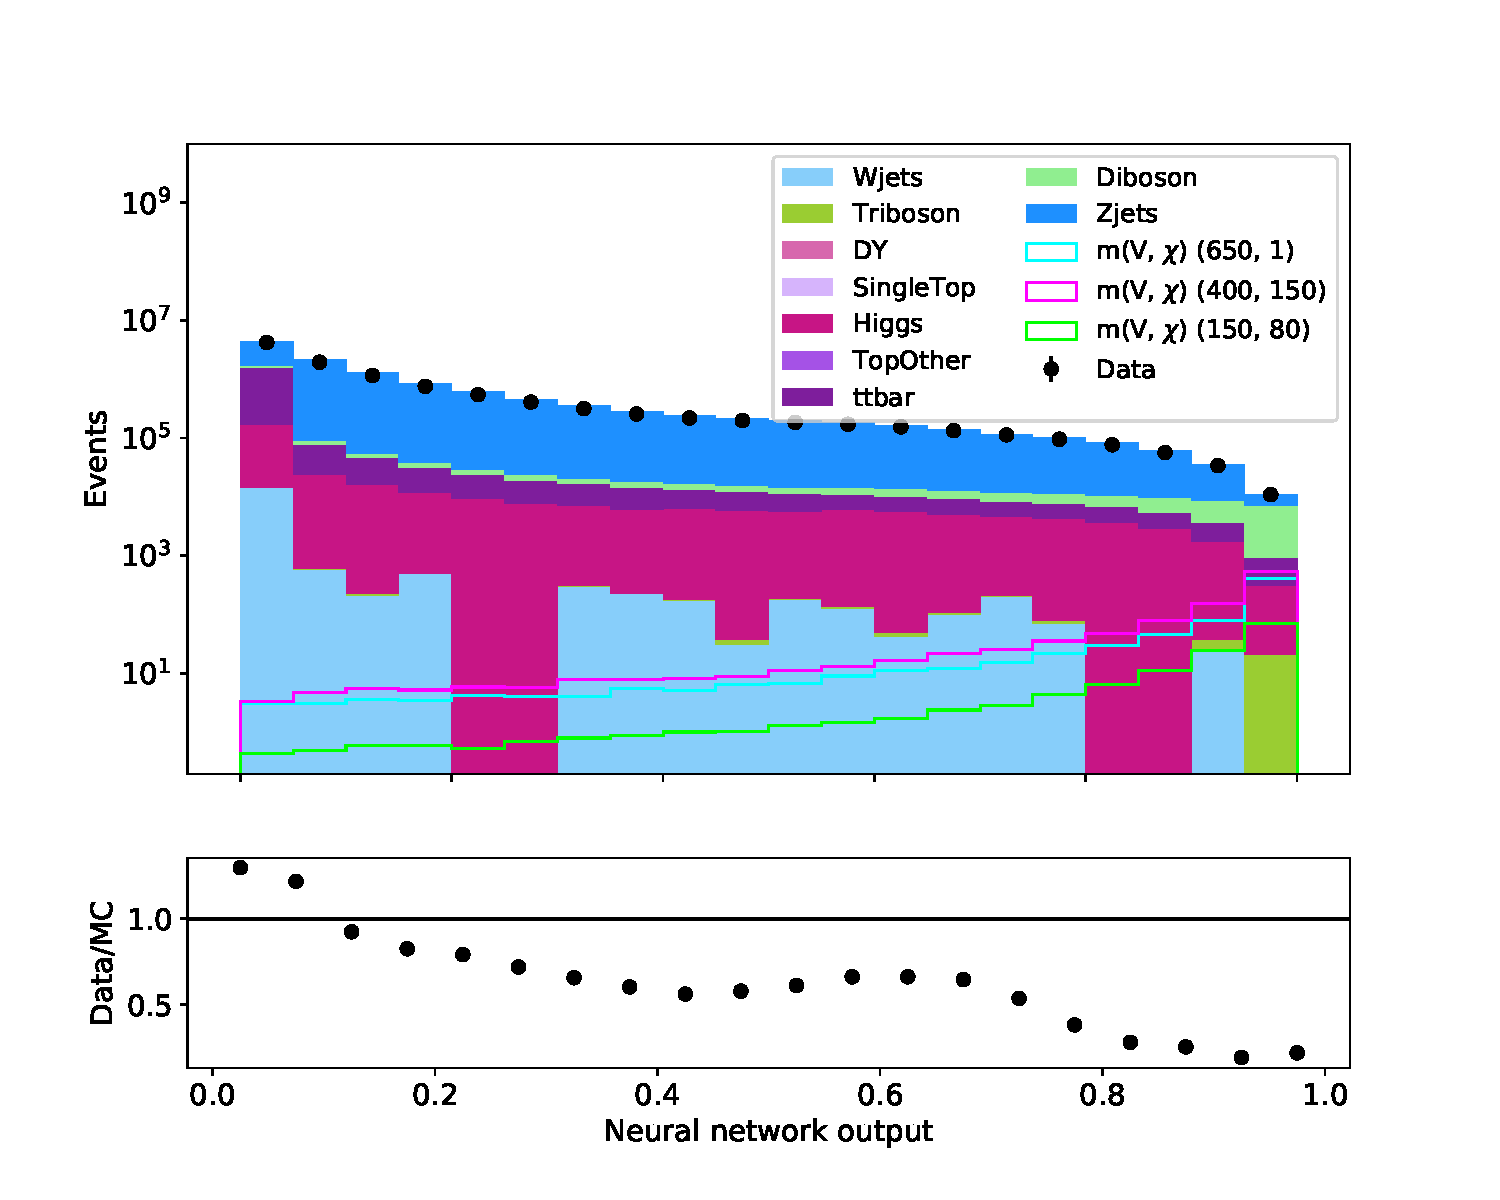
\includegraphics[width = \textwidth]{Figures/Stacked/stackedplot_NN_All_level_monoZ.pdf}
        \caption{Mono-Z.}
        \label{fig:MonoZNNLow}
    \end{subfigure}
    \caption{Test vs train for low mass splittings done with the NN. Here the test set is scaled up to match the number of training events.}
    \label{fig:AllLowNN}
\end{figure}


\begin{figure}[H]
    \centering
    \begin{subfigure}[t!]{0.49\textwidth}
        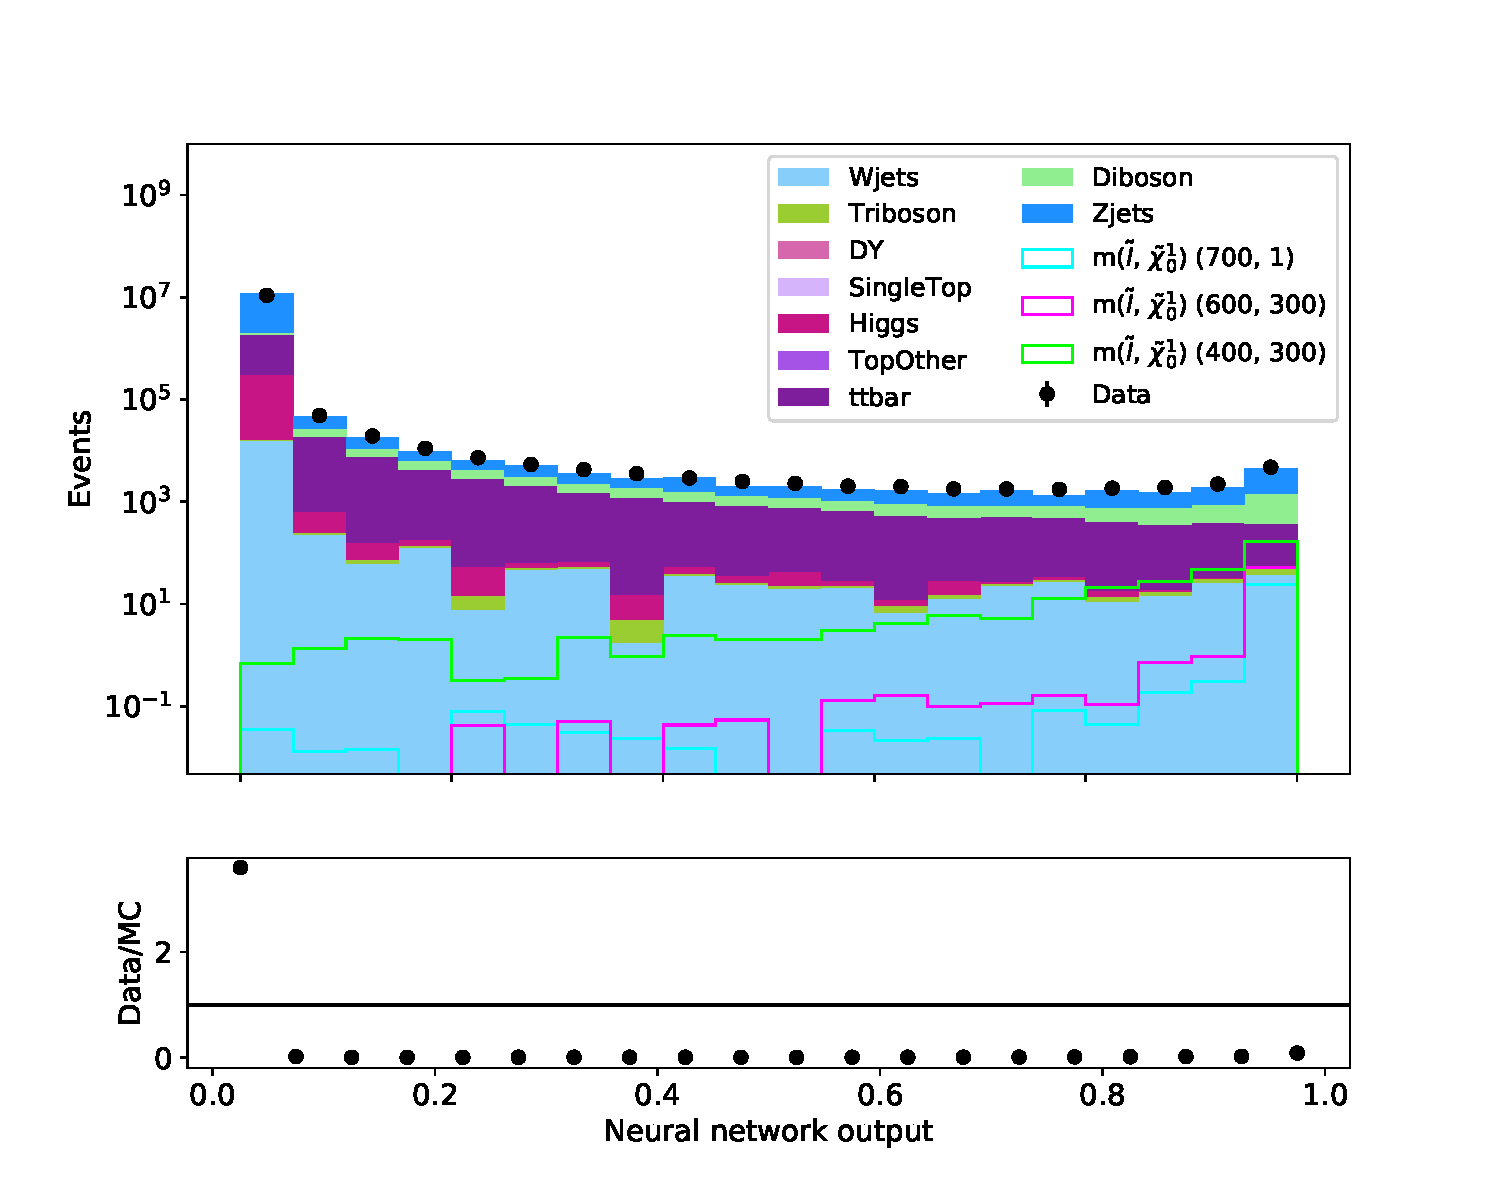
\includegraphics[width = \textwidth]{Figures/Stacked/stackedplot_NN_Low_level_slepslep.pdf}
        \caption{Direct slepton production.}
        \label{fig:SlepslepNNLow}
    \end{subfigure}
    \begin{subfigure}[t!]{0.49\textwidth}
        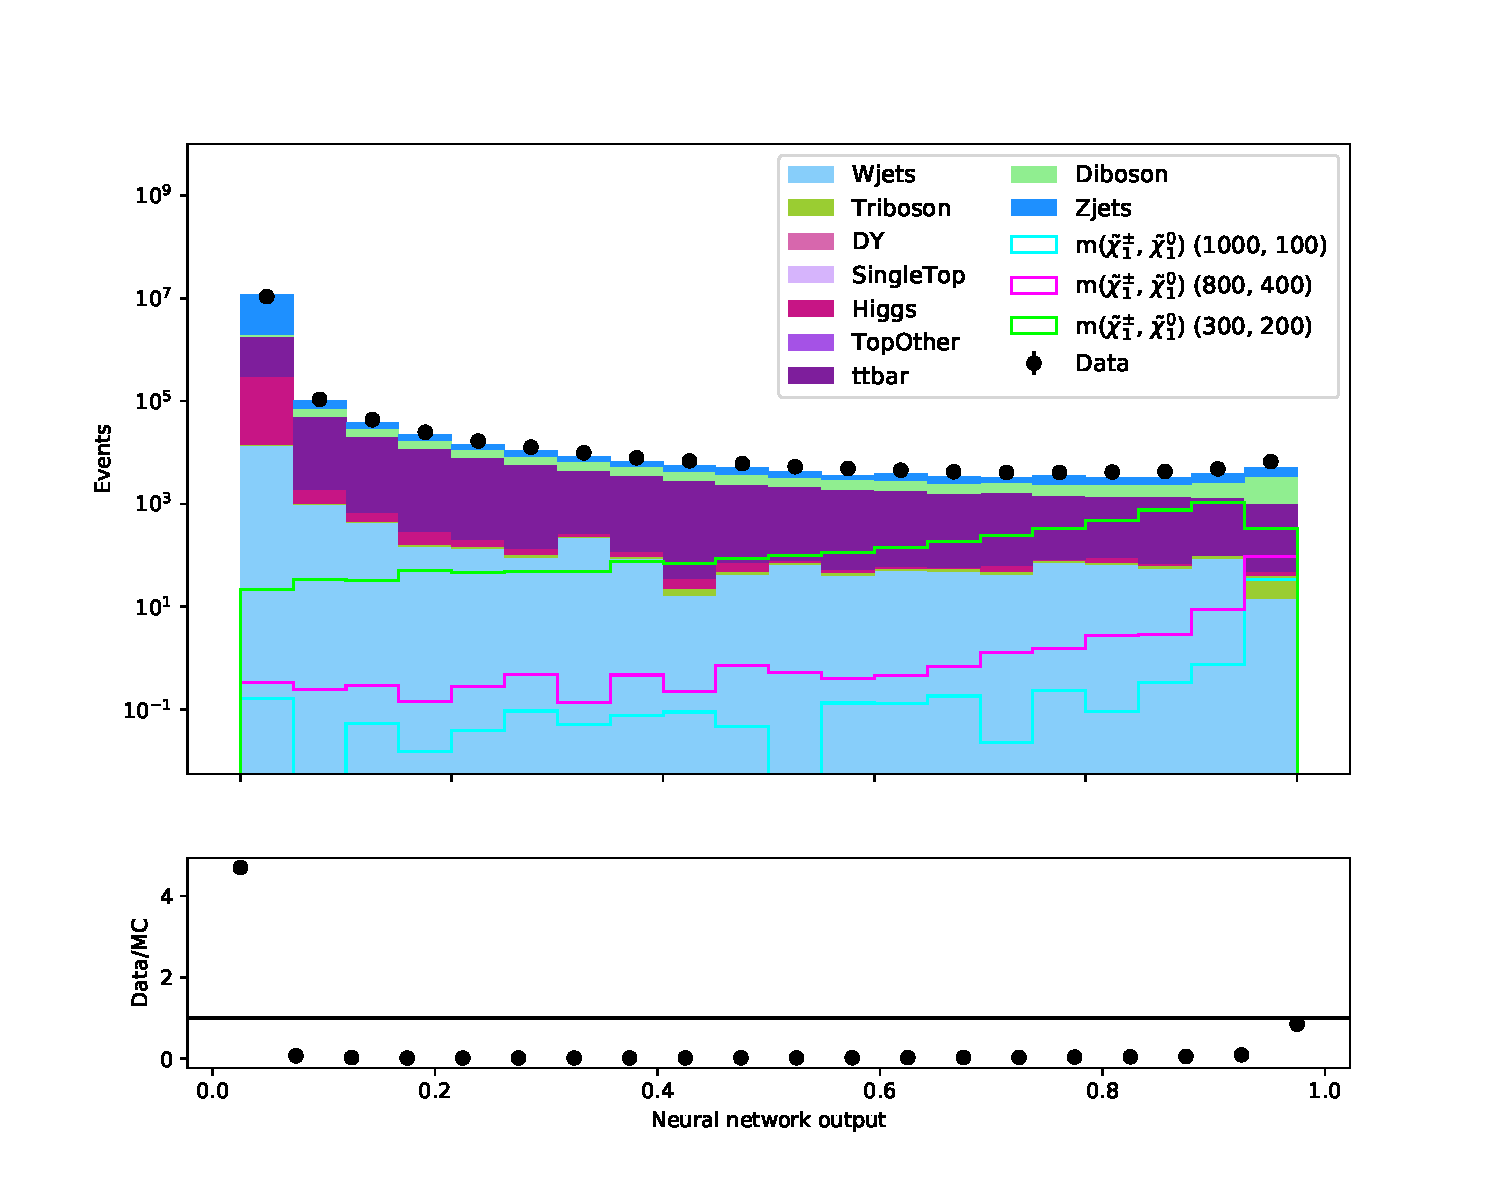
\includegraphics[width = \textwidth]{Figures/Stacked/stackedplot_NN_Low_level_slepsnu.pdf}
        \caption{Chargino production via $\Tilde{l}/\Tilde{\nu}$.}
        \label{fig:SlepsnuNNLow}
    \end{subfigure}      
    \begin{subfigure}[t!]{0.49\textwidth}
        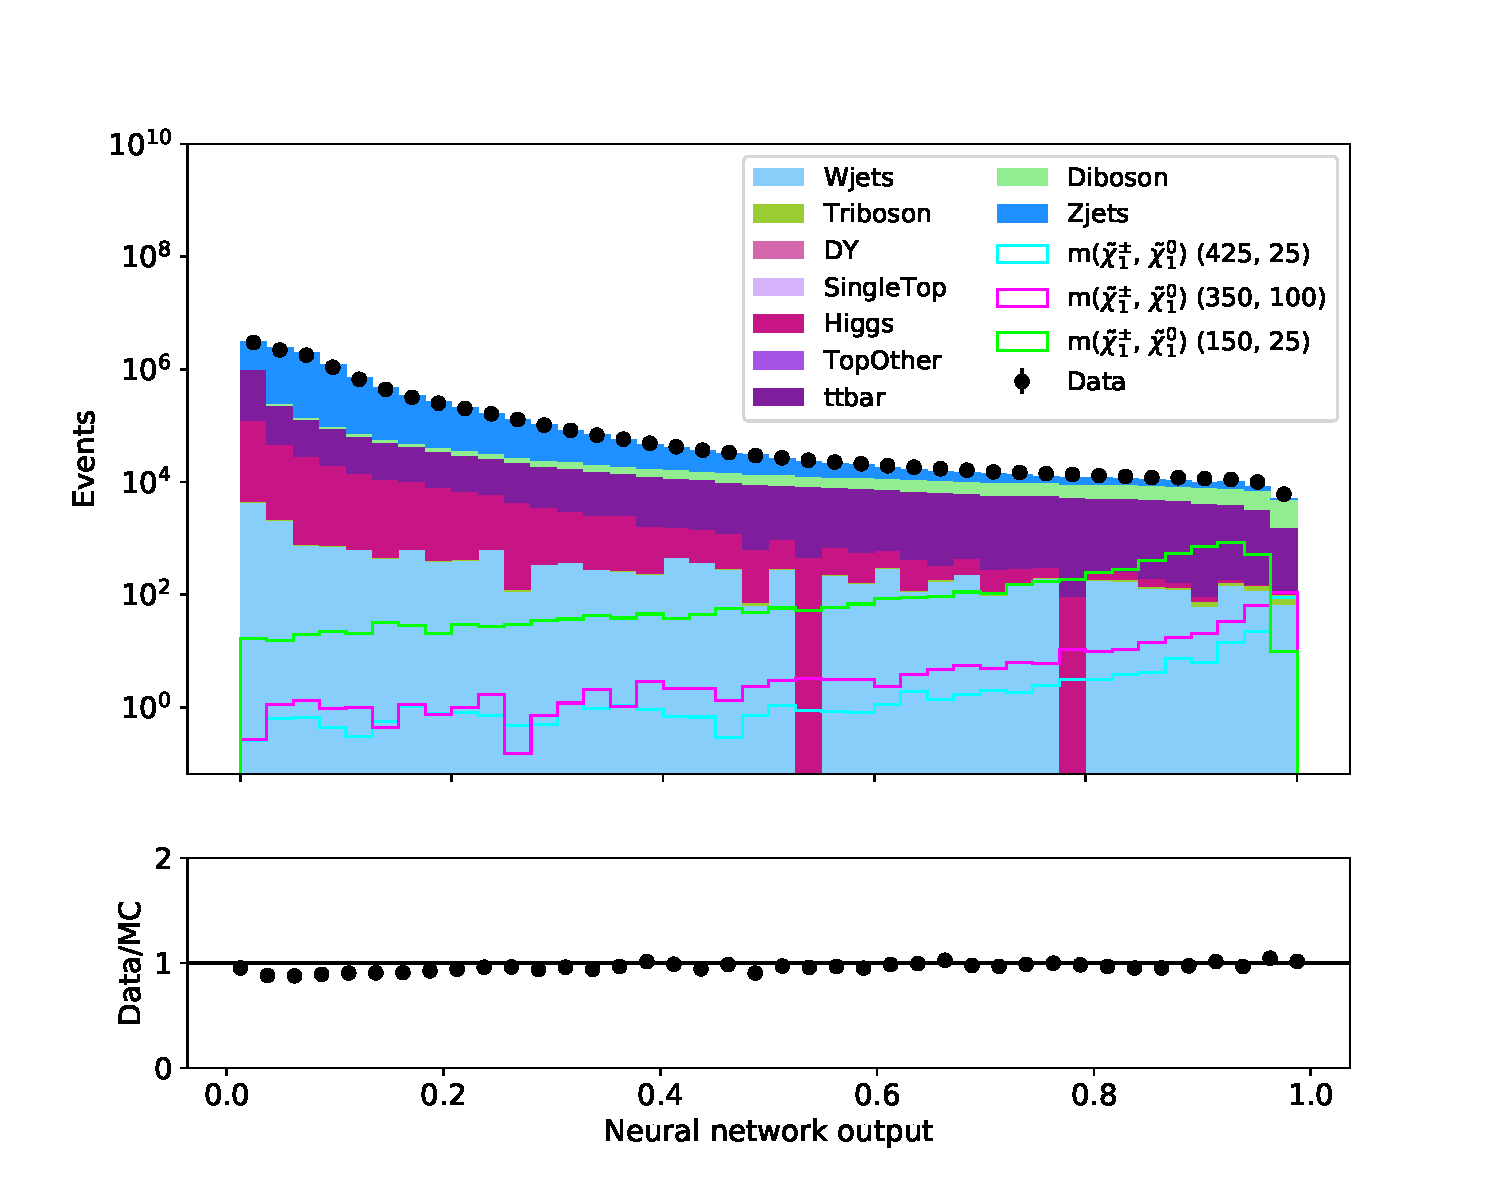
\includegraphics[width = \textwidth]{Figures/Stacked/stackedplot_NN_Low_level_WW.pdf}
        \caption{Chargino production via $W^\pm$.}
        \label{fig:WWNNLow}
    \end{subfigure}
    \begin{subfigure}[t!]{0.49\textwidth}
        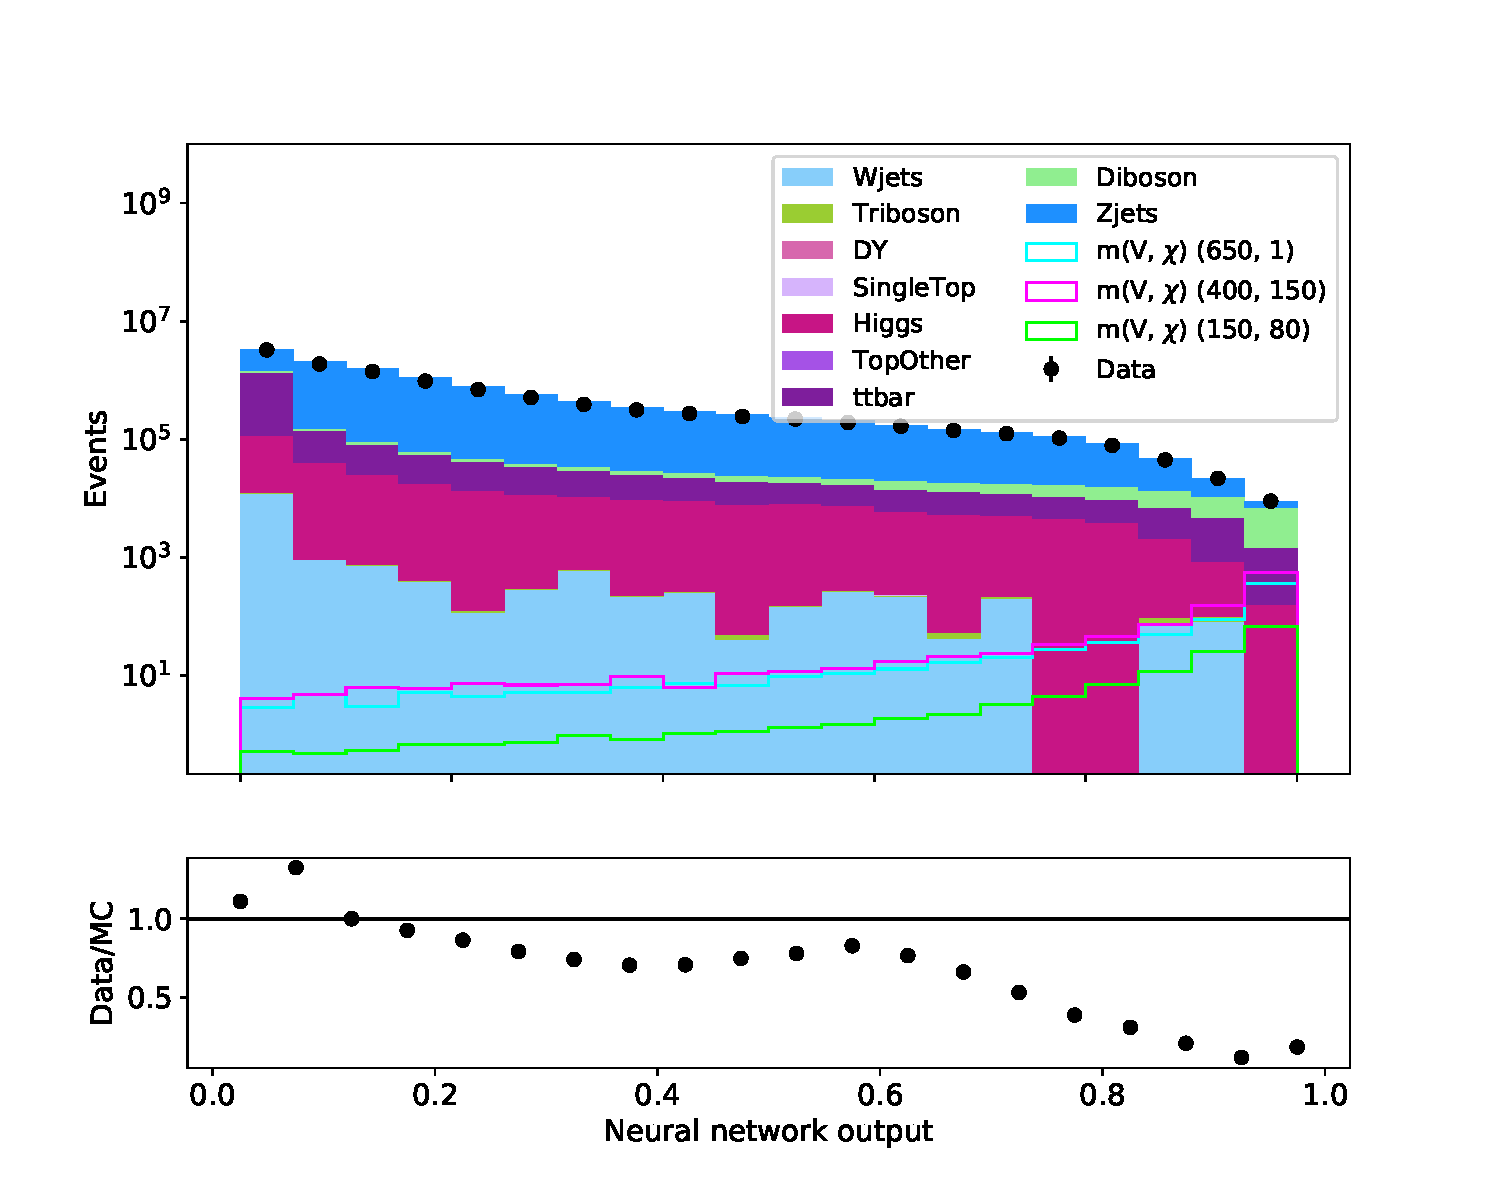
\includegraphics[width = \textwidth]{Figures/Stacked/stackedplot_NN_Low_level_monoZ.pdf}
        \caption{Mono-Z.}
        \label{fig:MonoZNNLow}
    \end{subfigure}
    \caption{Test vs train for low mass splittings done with the NN. Here the test set is scaled up to match the number of training events.}
    \label{fig:AllLowNN}
\end{figure}

\begin{figure}[H]
    \centering
    \begin{subfigure}[t!]{0.49\textwidth}
        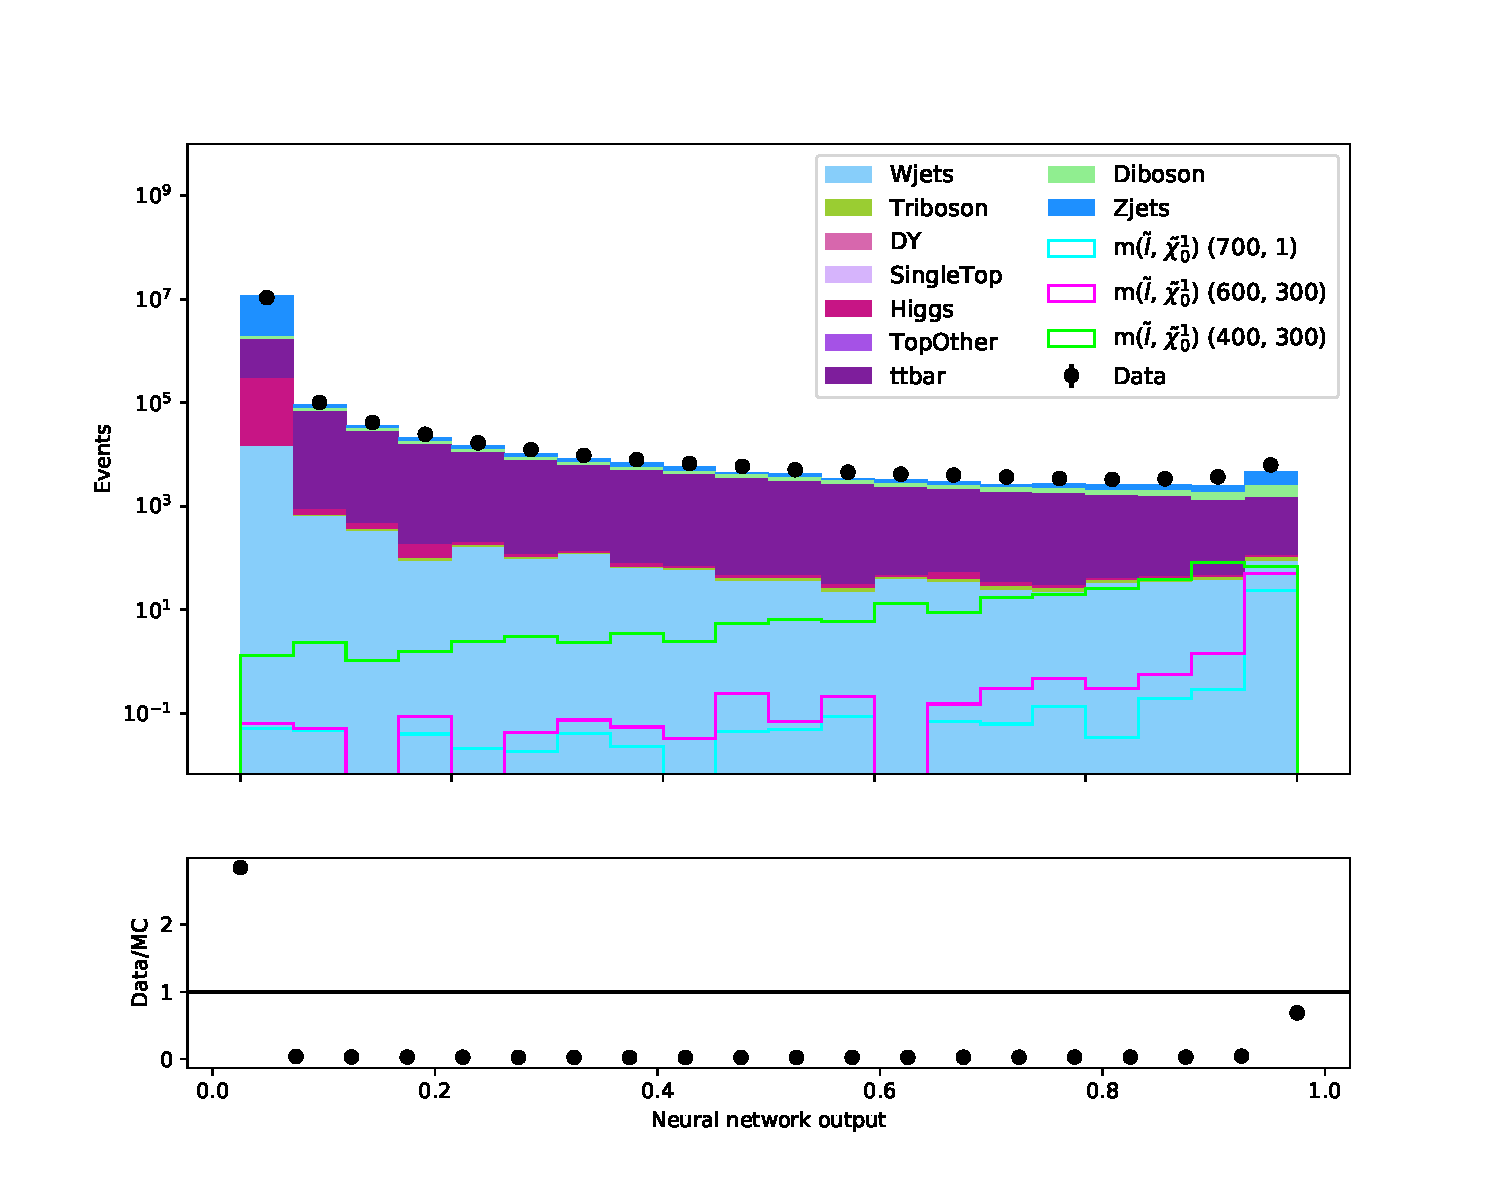
\includegraphics[width = \textwidth]{Figures/Stacked/stackedplot_NN_High_level_slepslep.pdf}
        \caption{Direct slepton production.}
        \label{fig:SlepslepNNLow}
    \end{subfigure}
    \begin{subfigure}[t!]{0.49\textwidth}
        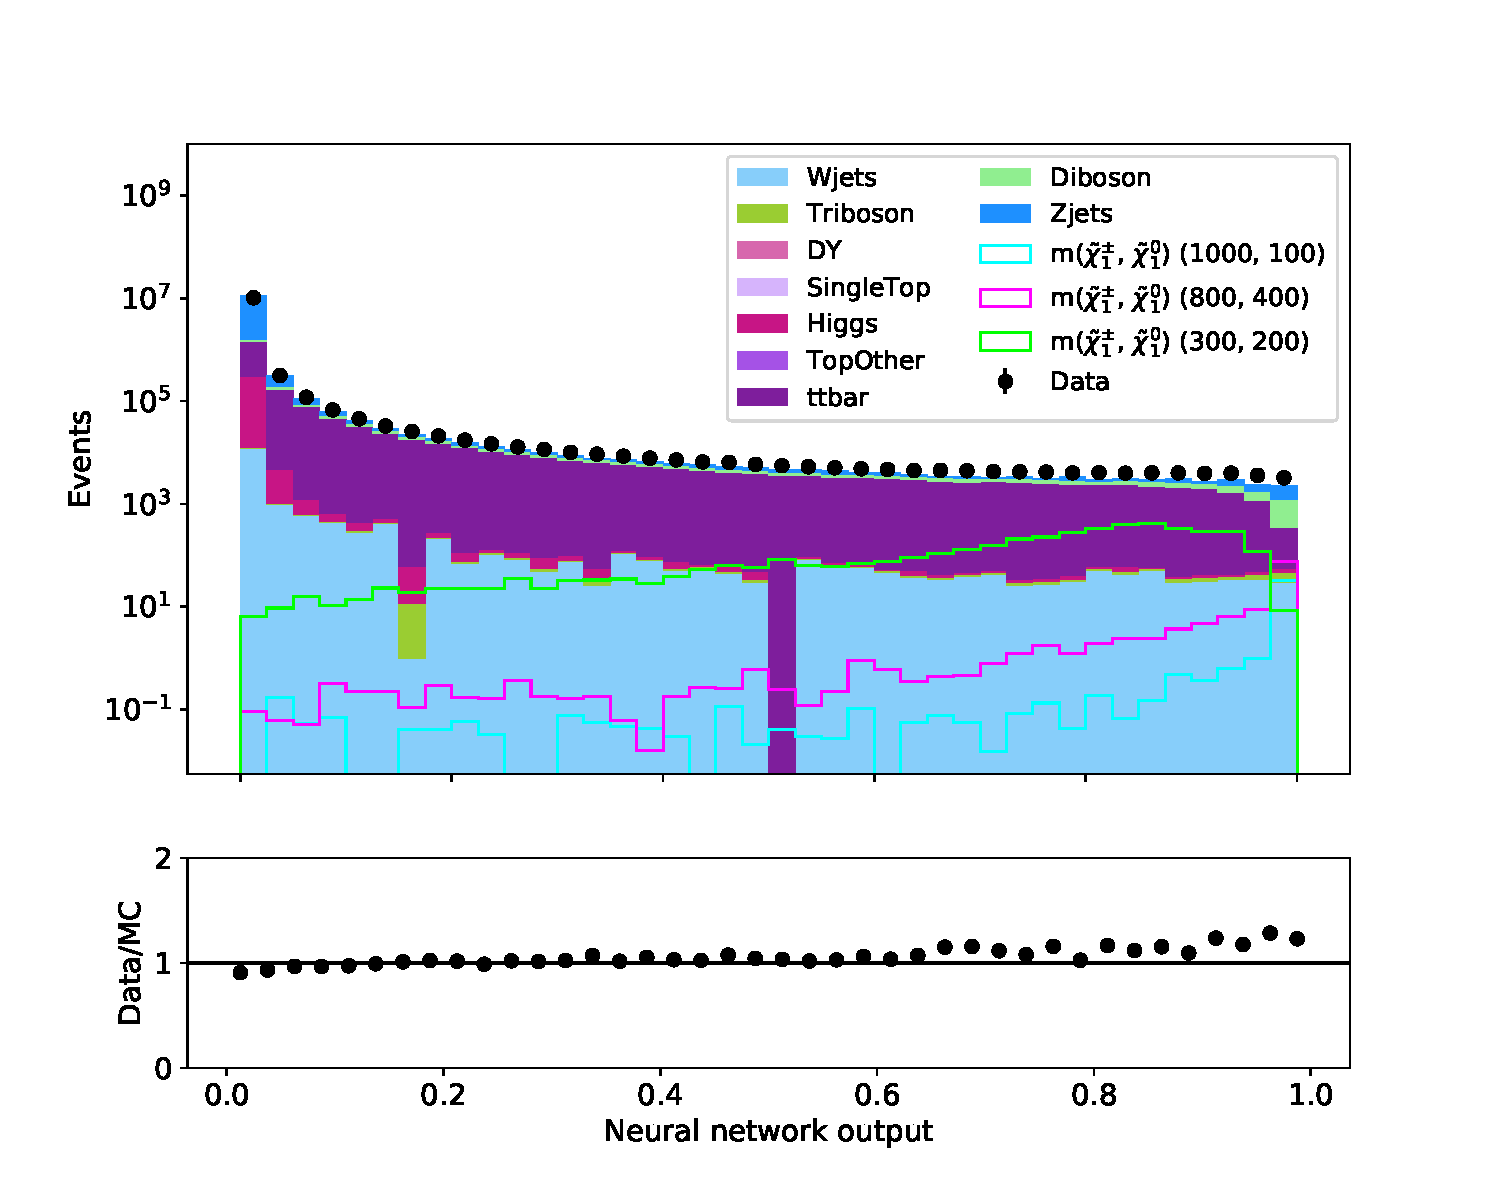
\includegraphics[width = \textwidth]{Figures/Stacked/stackedplot_NN_High_level_slepsnu.pdf}
        \caption{Chargino production via $\Tilde{l}/\Tilde{\nu}$.}
        \label{fig:SlepsnuNNLow}
    \end{subfigure}      
    \begin{subfigure}[t!]{0.49\textwidth}
        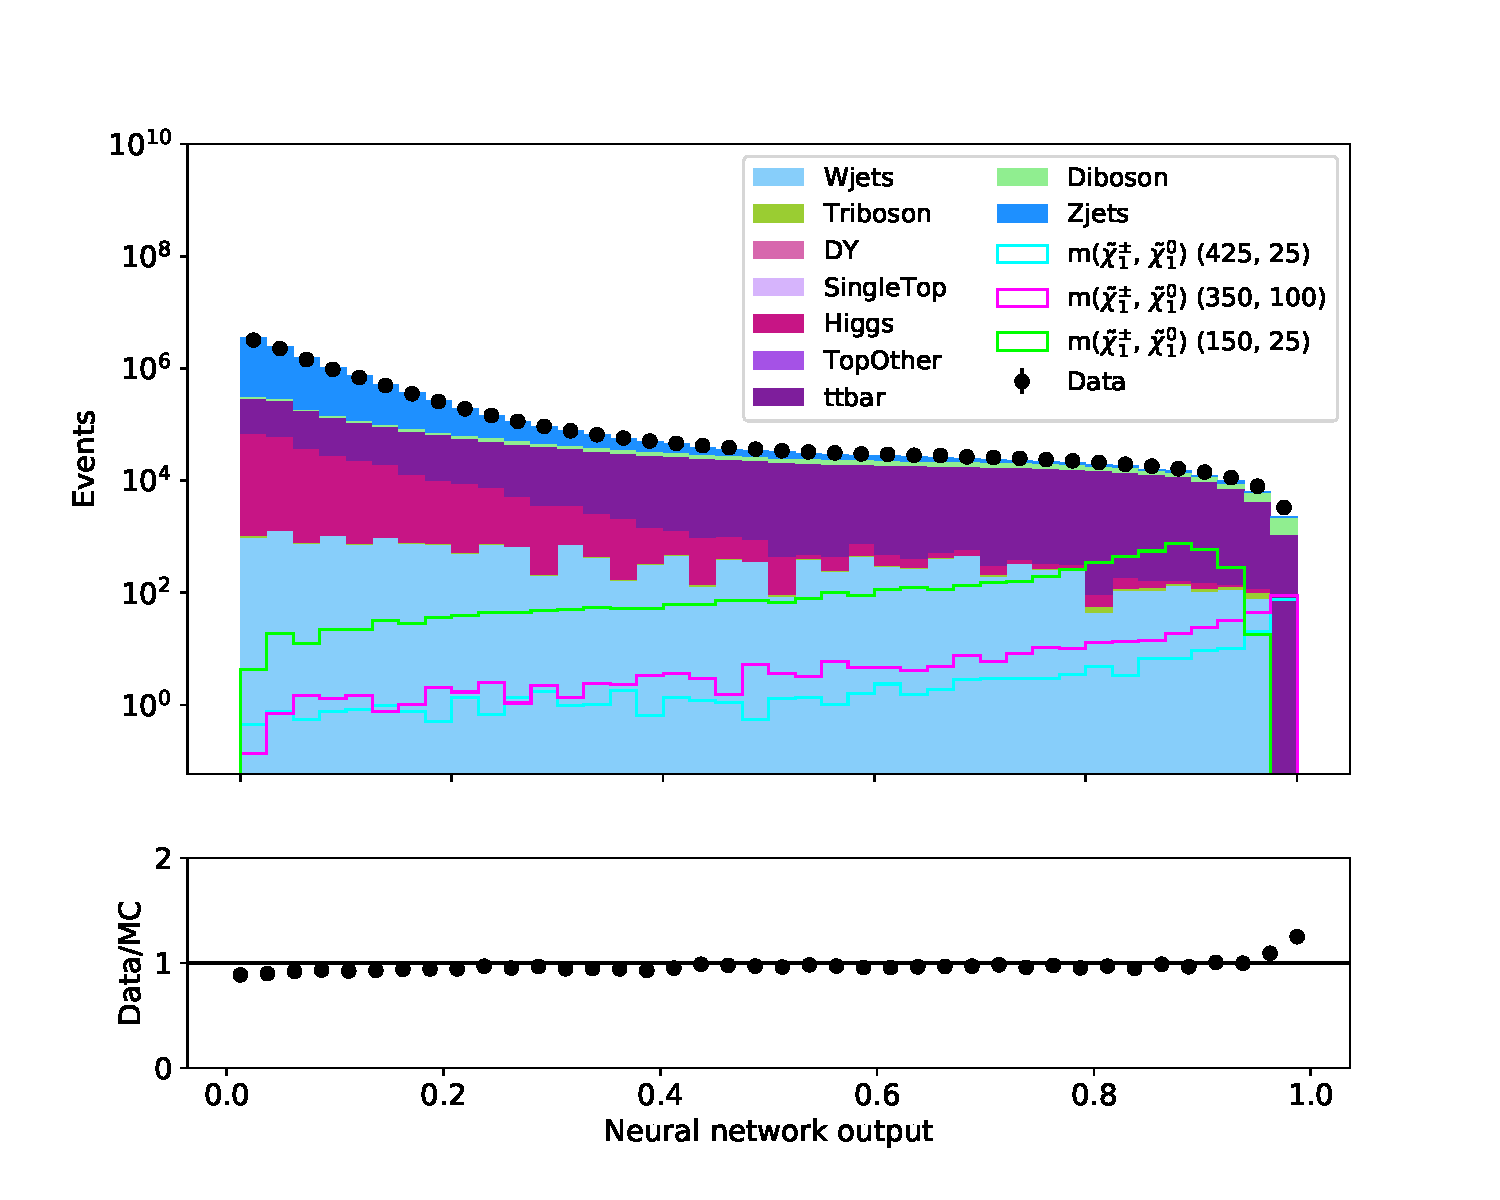
\includegraphics[width = \textwidth]{Figures/Stacked/stackedplot_NN_High_level_WW.pdf}
        \caption{Chargino production via $W^\pm$.}
        \label{fig:WWNNLow}
    \end{subfigure}
    \begin{subfigure}[t!]{0.49\textwidth}
        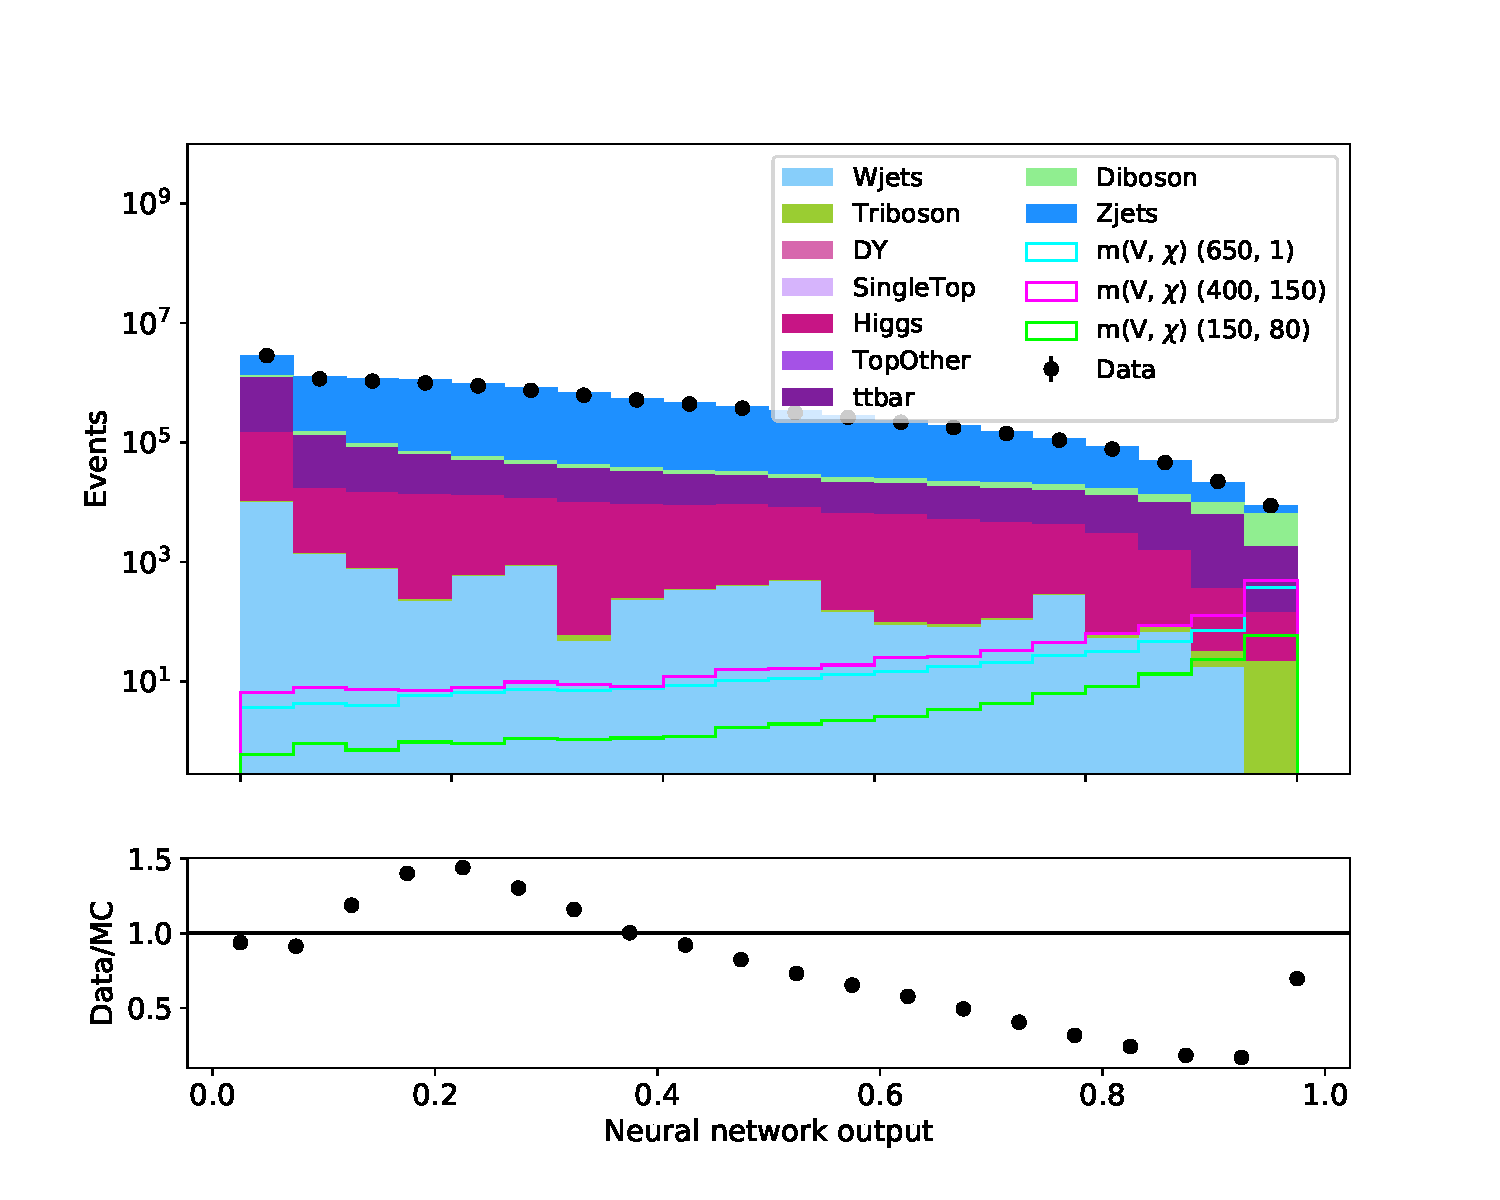
\includegraphics[width = \textwidth]{Figures/Stacked/stackedplot_NN_High_level_monoZ.pdf}
        \caption{Mono-Z.}
        \label{fig:MonoZNNLow}
    \end{subfigure}
    \caption{Test vs train for low mass splittings done with the NN. Here the test set is scaled up to match the number of training events.}
    \label{fig:AllLowNN}
\end{figure}



